\documentclass[12pt]{article}
\usepackage[margin = 1in]{geometry}
\usepackage[USenglish]{babel}
\usepackage{natbib}
\usepackage{multirow}
\usepackage{graphicx}
\usepackage{fancyhdr}
\usepackage{setspace}
\usepackage{verbatim}
\usepackage{booktabs}
\usepackage{amsmath}
\usepackage{lscape}
\usepackage{dcolumn}
\usepackage{subcaption}
\usepackage[title]{appendix}
\usepackage{xcolor}
\usepackage{todonotes}
\usepackage{titletoc}
\usepackage[colorlinks=true,citecolor=red!50!black,urlcolor=blue!50!black,linkcolor=red!50!black]{hyperref}

\author{Patrick W. Kraft\footnote{Ph.D. Candidate, Stony Brook University, \href{mailto:patrick.kraft@stonybrook.edu}{patrick.kraft@stonybrook.edu}.
%I thank Jennifer Jerit, Stanley Feldman, Yanna Krupnikov, Jason Barabas, Fridolin Linder, Scott Clifford, Peter DeScioli, Scott Bokemper, and participants of the Political Science Graduate Student Colloquium at Stony Brook University as well as participants at the panel of the 2015 Annual Meeting of the Midwest Political Science Association for helpful comments on earlier drafts of this paper.
}}
\date{today}

\title{Morals Don't Matter for Everyone\footnote{An earlier version of this paper was presented at the 73rd Annual Conference of the Midwest Political Science Association, April 16-19, 2015. The manuscript and code are available on GitHub: \url{https://github.com/pwkraft/mft}.}\\
\large{On the Conditionality of Moral Foundations in Political Reasoning}}
\date{\today}


\begin{document}
\maketitle
\onehalfspacing

\begin{abstract}
Moral Foundations Theory (MFT) proposes that political attitudes and ideology are structured by fundamental moral intuitions. While there is growing empirical support for theory in the social sciences, recent studies have critiqued key tenets of the theory (i.e., that moral intuitions are stable traits) as well as the measurement approach (i.e., self-reported judgements). The present paper contributes to the literature by exploring the conditions under which moral foundations are expressed in politics. Using open-ended survey responses in the 2012 American National Election Study, we utilize the Moral Foundations ``dictionary'' to identify references to basic moral intuitions when individuals report their attitudes towards political parties and candidates. The results show that the reliance on moral foundations in political reasoning is largely consistent with MFT. However, whether and how individuals evoke moral considerations is conditional on their political knowledge and exposure to political discourse. Overall, moral foundations have a powerful influence on public opinion and political behavior but this relationship is most evident among the politically knowledgeable---implying that moral reasoning is as much learned (from the political world) as it is innate. 

\vspace{\baselineskip}
\noindent \textbf{Keywords:} Moral Foundations Theory, Political Reasoning, Ideology, Political Behavior, Open-ended Survey Responses
\end{abstract}
\newpage


\section{Introduction}

% BASIC ARGUMENT:
% Open with debate about moral foundations and its usefulness for political science
% Recent crtics argue that it is less stable than it should be
% I argue that it is indeed less stable and that this instability is moderated by exposure to the political process.
% Morality as a way for people to justify their political preferences
% I look at how people justify their political preferences and whether they make references to moral foundations

To what extent do the public's political beliefs have a meaningful structure? This question has been of frequent scholarly interest in political science and related disciplines, yielding an array of different perspectives. Early accounts emphasized how ordinary citizens lack consistent political attitudes and knowledge necessary to form meaningful ideologies \citep[e.g.][]{converse1964nature}. However, with increasing levels of polarization and partisan sorting in contemporary politics \citep{iyengar2015fear}, there has been renewed interest in systematic psychological and attitudinal differences between liberals and conservatives \citep{jost2006end}. One such area of research focuses on the differing moral concerns of liberals and conservatives. According to \textit{Moral Foundations Theory} (MFT), moral thinking is organized by five innate intuitions: harm/care, fairness/reciprocity, ingroup/loyalty, authority/respect, and purity/sanctity \citep{haidt2008moral,graham2011mapping}. Liberals and conservatives differ in their relative emphasis of these foundations, with liberals prioritizing the foundations of harm/care and fairness/reciprocity, and conservatives endorsing all five dimensions more or less equally \citep{graham2009liberals}.\footnote{Subsequent accounts of MFT discussed the inclusion of further dimensions, such as \textit{Liberty/Oppression} \citep[c.f.,][]{graham2013moral,haidt2012righteous}. However, the analyses presented here will only focus on the dimensions initially suggested in \citet{haidt2008moral}.}

A series of studies builds on MFT and provides evidence for the influence of moral foundations on issue preferences \citep{koleva2012tracing, kertzer2014moral, low2015moral, clifford2015concerns}, candidate trait evaluations \citep{clifford2014linking}, and vote choice \citep{iyer2010beyond, franks2015using}. However, recent research cast some doubt on the theory's basic tenets \citep[e.g.,][]{suhler2011can}. \citet{smith2016intuitive} empirically investigated three implicit assumptions underlying MFT, namely that moral foundations are individual traits that are relatively stable over time, that changes in moral foundations predict changes in political ideology, and that the foundations are heritable. The empirical evidence provided by \citet{smith2016intuitive} does not support these assumptions, but this critique stands in contrast to the growing body of work that documents the political relevance of moral foundations. The present study attempts to reconcile this contradiction by taking a different tack and directly examining the conditions under which the moral foundations are consequential to a person's political judgments. Indeed, \citet{smith2016intuitive} conclude that their findings are ``consistent with the notion of moral foundations being highly responsive to context: more of a state than a trait.'' Yet, few studies systematically investigated the conditionality of the relationship between moral foundations and political attitudes \citep[see][for a notable exception]{clifford2015concerns}.

The present study provides a first step in this direction by directly analyzing the degree to which individuals vary in the expression of moral concerns in political reasoning and judgment. Using data from the 2012 American National Election Study, we create a measure of moral reasoning based on individual responses to the open-ended likes-dislikes questions and the moral dictionary introduced by \citet{graham2009liberals}. Relying on open-ended questions rather than traditional survey-based measures of moral foundations allows us to investigate patterns of moral reasoning among individuals where the potential connection between morality and politics is not induced or facilitated by design.

The analyses reveal systematic differences between liberals and conservatives in their reliance on specific moral considerations when evaluating political parties and candidates even without being cued to think about morality.
These differences, in turn, affect political evaluations as well as voting behavior---even after controlling for a person's party identification. Most importantly, the overall reliance on moral foundations in political judgment as well as the respective differences between liberals and conservatives are conditional on knowledge and exposure to political discourse. Even though the ideological differences are broadly consistent with MFT, moral reasoning in the realm of politics is more context-specific than previous research suggests. From a methodological standpoint, the present study introduces techniques to improve the analysis of open-ended survey responses and illustrates their value to illuminate the antecedents of political reasoning.


\section{Theoretical Framework}

Moral values serve as a source for coherence in political attitudes and they shape individual belief systems. There is evidence, for example, that moral considerations predict a person's attitudes on a range of ``culture-war'' issues such as abortion and same-sex marriage above and beyond demographic characteristics and ideology (\citealt{koleva2012tracing}; also see \citealt{clifford2015concerns}). Even issues that are not considered intrinsically ``moral,'' such as those related to the economy, can be connected to underlying moral convictions \citep{ryan2014reconsidering}. Moral convictions, in turn, have been shown to reduce tolerance of divergent attitudes and lower acceptance of compromise \citep[][]{skitka2010psychology,ryan2016no}. As such, individual moral reasoning may provide important insights into the recent increase in polarization in American Politics \citep{iyengar2015fear}.


\subsection{Moral Foundations Theory}

One major focus of the moral foundations framework is the relationship between moral values and political belief systems \citep[c.f.,][]{haidt2012righteous}. Liberal morals have been shown to focus on ``individualizing'' foundations, which include harm/care and fairness/reciprocity. Conservatives, on the other hand, also emphasize the remaining foundations of ingroup/loyalty, authority/respect, and purity/sanctity, labeled the ``binding'' foundations \citep{haidt2007morality,graham2009liberals}. Haidt and colleagues developed the Moral Foundations Questionnaire (MFQ) to measure individual differences in the emphasis of each foundation. The MFQ consists of a series of items that explicitly ask people to rate the relevance of different considerations when making decisions about right and wrong.\footnote{For example, one of the considerations is ``Whether or not some people were treated differently than others.'' High relevance of this statement is viewed das an indicator for the fairness/reciprocity dimension (c.f., \url{http://www.moralfoundations.org/}).} The questionnaire also asks individuals to indicate their level of agreement with statements that represent the values implied by the five foundations.\footnote{For example, respondents are asked to report their agreement with the statement ``I am proud of my country's history'' as an indicator for the ingroup/loyalty dimension.}

Relying on the MFQ, subsequent research extended the initial findings. For example, scholars showed that moral concerns predicted attitudes towards a wide variety of divisive political issues \citep[e.g.][]{koleva2012tracing,kertzer2014moral,low2015moral}. \citet{federico2013mapping} linked moral foundations to individual social dominance orientation (SDO) and right-wing authoritarianism (RWA). Further research directly investigated the relationship between moral foundations and candidate preferences \citep{iyer2010beyond} or trait inferences about candidates \citep{clifford2014linking}. Moral foundations have also been shown to predict turnout \citep{johnson2014ideology} as well as voting behavior in the 2012 US Presidential election \citep{franks2015using}. Overall, this research strongly supports the view that liberals and conservatives endorse different moral foundations and that these differences are related to political attitudes, evaluations, and behavior.

\citet{smith2016intuitive}, on the other hand, used the MFQ to examine some basic assumptions underlying MFT using data from several twin panels. The authors investigated whether moral foundations can be viewed as stable traits that vary little over time, whether changes in moral foundations predict changes in ideology (or vice versa), and whether there are sufficient signs of heritability in the emphasis of moral foundations. Overall, the evidence reported in \citet{smith2016intuitive} seems to contradict MFT: the foundations are less stable than ideology, do not seem to predict changes in the latter over time, and do not seem to be inherited through genes. However, it should also be noted that the analyses presented by \citet{smith2016intuitive} are not without limitations. For example, their analyses of stability over time relied on different sub-scales of the MFQ in each of the waves, which might induce some of the instability between waves in the sample. Nevertheless, the results raise the possibility that the relationship between ideology and moral foundations might not be as stable as initial research suggested.

As such, directly investigating the conditions under which moral reasoning occurs when people think about politics might shed some light on the divide between the growing body of research highlighting the influence of the MFT on political attitudes and work challenging those conclusions \citep[e.g.][]{smith2016intuitive}. As we will argue below, this step involves measuring moral foundations in political reasoning without relying on the MFQ, which has been used in nearly all existing work \citep[but see][]{clifford2014linking}.


\subsection{The `Missing Link' to Political Reasoning}

While many studies report consistent differences between liberals and conservatives in terms of their latent emphasis on moral foundations, recent research points to the instability of moral foundations and their relationship with ideology. In an attempt to reconcile this apparent contradiction, we examine whether people utilize the foundations in their day-to-day political reasoning (i.e., without being prompted by the language of a questionnaire). Previous research has relied almost exclusively on the Moral Foundations Questionnaire (MFQ), which explicitly asks people to judge the relevance of particular moral considerations \citep[e.g.][]{graham2011mapping}. However, by directly asking people about the importance of considerations related to the five foundations, previous analyses presuppose an important link that requires more careful empirical investigation. The present study addresses this gap by examining whether differences in moral reasoning between liberals and conservatives manifest themselves in a more unobtrusive context (i.e., without explicitly asking people to think about morality).

Measuring moral foundations using the MFQ imposes important constraints on our theoretical conceptualization of moral reasoning and the range of hypotheses we can investigate. Most importantly, it does not allow us to directly examine the conditions under which the connection between moral values and political ideology manifests itself when citizens reason about politics and evaluate political actors. Some scholars have criticized the MFQ because it does not ask people to make moral judgments per se \citep[e.g.][]{clifford2015moral}. Indeed, \citet[1031]{graham2009liberals} describe the reports on moral relevance as ``self-theories of moral judgment,'' rather than direct measures of judgment itself. Such abstract self-theories might, in turn, deviate from actual judgments in specific situations.

From a theoretical perspective, moral foundations are viewed as stable traits that affect attitudes and preferences regardless of potential individual differences and contextual effects. However, the incorporation of moral considerations in a specific political context could be much more variable. Previous research suggests that campaigns and elite communication can have important influences on individual moral reasoning. For example, \citet{clifford2013words} found that at the elite level, proponents and opponents of stem cell research place distinctive weights on moral foundations which in turn affected the public attitudes and the underlying considerations related to the issue. A subsequent study showed that elite rhetoric plays an important role in linking individual moral foundations with political attitudes, but only for those individuals who were most likely be exposed to it (\citealt{clifford2015concerns}; also see \citealt{day2014shifting}). While these studies do not contradict MFT, they cast some doubt on the notion that moral reasoning in politics is as a direct reflection of stable moral intuitions. 

The literature on \textit{moral convictions} further suggests that moral reasoning in the realm of politics can be more variable than proposed by MFT. Skitka and colleagues argue that individuals hold moralized attitudes if they have a universal perception of ``right and wrong'' connected to the issue at hand \citep{skitka2005moral,mullen2006exploring,skitka2010psychology}. This view implies that there can be considerable variance in the degree to which moral considerations are raised between individuals and across issues. However, the MFQ measures moral foundations as general traits that are implicitly assumed to apply in any context. Moving beyond the MFQ and measuring moral reasoning as the explicit expression of foundations allows us to directly examine the degree to which political attitudes are infused by moral convictions.

Overall, individuals who are exposed to the political process and resulting elite communications are more likely to incorporate moral considerations in their political reasoning because they adopt the respective arguments from elite discourse. Individuals who are not engaged in politics, on the other hand, might focus on other considerations when forming their preferences. The extent to which individuals rely on moral considerations when evaluating political actors is therefore not necessarily stable among individuals and across contexts. Rather, the tendency to emphasize moral foundations may be contingent upon individual levels of political knowledge, media exposure and political discussions.\footnote{Other scholars contend that the reliance on basic values is not contingent on individual characteristics such as political sophistication \citep[e.g.][]{feldman1992political,goren2001core,goren2004political,marietta2007values}.} The degree to which political attitudes are moralized as well as the ideological differences in moral reasoning cannot be investigated by relying solely on the MFQ. Instead, it is necessary to differentiate between a person's tendency to endorse a moral \textit{foundation} (as a stable trait), and moral \textit{reasoning} as the actual reliance on specific moral considerations and arguments in specific political judgments. Previous research has largely neglected this difference.


\section{Empirical Analyses}

% NEW ANALYSES:
% 1a: Differences in Moral Foundations are similar to other research
% 1b: Differences in Moral FOundations predict candidate evaluations and vote choice
% 2a: The degree to which moral foundations are raised is conditional on campaign exposure and political engagement
% 2b: Campaign exposure influences the difference between liberals and conservatives

Insofar as moral intuitions play a role in political reasoning, citizens should rely on the moral foundations when reporting their attitudes towards political actors, even if they are not explicitly asked to do so. Thus, the first step of the analyses will be to replicate the findings connected to MFT and ideology using open-ended survey responses to general questions about political preferences. We expect that liberals will be more likely to spontaneously mention the moral foundations of harm/care and fairness/reciprocity than conservatives when evaluating political parties and candidates. Conversely, conservatives will be more likely to emphasize moral foundations of ingroup/loyalty, authority/respect, and purity/sanctity than liberals. Moral reasoning measured through open-ended responses is further expected to be politically consequential. The differences in the degree to which each foundation is emphasized should directly affect political preferences and vote choice consistent with the propositions of MFT.

After replicating the basic findings in the MFT literature in a more unobtrusive survey context that does not evoke issues of morality, the present study contributes to the literature by clarifying the role of the foundations in day-to-day reasoning. We expect that individuals who are more exposed to political discourse and more engaged in politics will be more likely to emphasize moral foundations when evaluating political parties and candidates than those who have less experience and are less politically engaged. Furthermore, these differences are expected to exacerbate the ideological divide in moral reasoning.


\subsection{Data, Variables, and Model Specification}

The analyses presented here are based on the 2012 American National Election Study, which contains two representative cross-sectional samples. One sample was conducted by computer assisted face-to-face interviews while the other sample is based on an internet panel group. Both samples are pooled in the analyses. While each consisted of a pre-election and a post-election wave, most items described below are drawn from the pre-election wave.\footnote{The open-ended items were included only in the pre-election wave. Accordingly, wherever possible, the set of explanatory variables was limited to the pre-election wave.}

The major dependent variables are based on open-ended questions in which respondents were asked to report what they \textit{liked} and \textit{disliked} about either presidential candidate as well as the Republican and Democratic parties. More specifically, respondents were asked to list anything in particular that they like/dislike about the Democratic/Republican party as well as anything that might make them vote/not vote for either of the Presidential candidates and were probed by the interviewer asking ``anything else?'' until the respondent answered no. The responses to the eight open-ended like/dislike questions (evaluating both parties and both candidates) were aggregated for each individual and pre-processed by correcting spelling errors using an implementation of the Aspell spell checking algorithm in \texttt{R} (\url{www.aspell.net}).

Respondents were not included in the analysis if they failed to provide an answer to all open-ended items, or if the interview language was Spanish. Table~\ref{tab:app_mis} in the appendix provides an overview over the number of omitted cases. About 4\% of the interviews were held in Spanish and about 7\% of the respondents did not provide any open-ended response. Furthermore, Figure~\ref{fig:appB2num} in the appendix displays histograms of the length of the respondents' answers to all open-ended items. On average, the collection of all open-ended responses consists of about 75 words for each individual.

Our goal is to use the open-ended responses to identify the extent to which respondents relied on specific moral foundations when talking about their political attitudes and preferences. We use the dictionary created by \citet{graham2009liberals} that identifies references to specific moral foundations. Other studies in the domain of MFT relied on a similar dictionary to investigate moral considerations in news media coverage about stem cell research \citep{clifford2013words}.\footnote{The dictionary provided by \citet{graham2009liberals} is also presented in Appendix~\ref{app:oview}.} In the present research, we use the same dictionary to analyze open-ended survey responses. Words like ``protect'' and ``suffer'' indicate references to the harm/care foundation, ``equality'' and ``tolerant'' signal reasoning based on the fairness/reciprocity foundation, ``patriot'' and ``betrayal'' indicate reference to the ingroup/loyalty foundation, ``honor'' and ``respect'' signal considerations related to authority/respect, whereas ``integrity'' and ``duty'' indicate reference to the purity/sanctity foundation.

\citet{graham2009liberals} developed the word lists as a collection of general associations related to the foundations that could be applied in any context. However, some words might be problematic when applied to the open-ended responses considered here. In particular, certain words might be too ubiquitous in the realm of politics and candidate evaluations to be regarded as an unambiguous indicator for specific moral considerations. For example, the moral foundations dictionary includes ``leader,'' ``duty,'' and ``honor'' as signal words for the authority/respect dimension. Should all three words be considered as equally indicative of the respective foundation? After all, if respondents are asked about their attitudes towards both presidential candidates, they might be inclined to describe them as good or bad \textit{leaders} irrespective of explicit moral considerations related to authority. If that is indeed the case, the term ``leader'' should appear more frequently in open-ended responses across all individuals.

Conventional dictionary-based methods consist of dichotomous indicators or simple counts of signal word occurrences for each dictionary category in each text or response. As such, the only way to address this problem using conventional methods would be to revise the dictionary and eliminate words that are deemed problematic. However, this leaves a lot of discretion to the researcher. Instead, we rely on techniques developed in the fields of information retrieval to match search queries to relevant text documents \citep[see][for an introduction]{manning2008introduction}. In that context, when a search engine identifies the set of documents most relevant to a query, it increases the importance of keywords that appear in fewer documents since those terms carry more discriminative information. 

We rely on the same logic to create a measure (referred to below as ``similarity score'') that represents the degree to which a person's open-ended response resembles Graham et al.'s \citeyearpar{graham2009liberals} dictionaries for each moral dimension, while increasing the importance of more informative or discriminatory words in the dictionary. Formally, ``similarity'' is the tf-idf cosine score between the dictionaries and a person's response to the open-ended items on the ANES\footnote{The acronym tf-idf stands for ``term frequency - inverse document frequency,'' which refers to the rationale that the frequency of specific terms are weighted by the inverse of the frequency of occurrence across documents.}. A technical discussion appears in Appendix~\ref{app:measure}, but the measure has several useful properties that we note here. The similarity score is a continuous measure that ranges between 0 (no overlap between dictionary and response) and 1 (response is identical to dictionary), and is independent of response length. The score increases if more words in the dictionary appear in a given response. Most importantly, however, words that appear in nearly all open-ended remarks affect similarity less than the words mentioned only by few respondents (because ubiquitous words convey less information about differences across individuals). 

Overall, the similarity score provides a correction for potential distortions due to suboptimal terms in the dictionary while leaving its exact content outside of the researcher's discretion. While the resulting measure theoretically ranges from 0 to 1, we only observe very low values since open-ended responses are naturally quite distinct from the raw dictionaries. Since the exact values do not have a straightforward interpretation, the measure for each moral dimension is rescaled to unit variance\footnote{Technically, values on this variable describe the cosine of the angle between the tf-idf vector space representation of the dictionary and each open-ended response. Please refer to the Appendix~\ref{app:measure} for a more detailed discussion.}.

Due to the fact that the similarity scores are bound at zero (i.e. none of the words in the dictionary appear in the response), individual response patterns are modeled via Tobit regressions for each of the moral foundations under consideration. As will be further described below, the Tobit framework allows us to decompose the estimates into the effect on the probability of mentioning a specific foundation \textit{at all} as well as the degree of emphasis on the foundation given that it was mentioned by a respondent \citep[see][for details on the decomposition of Tobit model estimates]{mcdonald1980uses}. The key independent variable used to predict the emphasis on each of the moral foundations, is \textit{political ideology}. Respondents were asked to place themselves on a seven-point scale ranging from extremely liberal to extremely conservative. Since there is no reason to suggest that moderates should fall in between liberals and conservatives in terms of their moral foundations (i.e. that the relationship between `continuous' ideological self-placement and the likelihood to mention specific moral foundations is inherently linear), we constructed dichotomous variables indicating whether respondent identified as liberals, conservatives, or moderates.

Additional control variables included in the analyses are \textit{church attendance}, \textit{education} (college degree), \textit{age}, \textit{sex}, \textit{race} (African American), survey mode (online vs. offline), as well as the overall length of the individual responses in the open-ended questions (\textit{measured as logged number of words}). The inclusion of the length of individual responses as control variables should account for potential confounding factors such as general effects of increased political literacy on the complexity of open-ended responses.

In order to examine the relevance and consequences of moral reasoning, the similarity scores for each of the moral foundations are used as independent variables to predict political outcomes. The dependent variables considered here are \textit{candidate} and \textit{party evaluations} (measured as the respective feeling thermometer differentials), as well as \textit{voting behavior} (measured as a dichotomous indicator of vote choice for the Democratic rather than the Republican Presidential candidate reported in the post-election wave). In addition to the controls discussed previously, these analyses include measures of \textit{party identification}, which were recoded similarly to ideology.

The final set of analyses investigates whether the expression of moral considerations in political judgment is conditional on knowledge and exposure to political discourse. The factors that are therefore expected to be related to references to moral foundations include \textit{political knowledge}, which was measured as the sum of correct answers to objective knowledge questions. The analysis also investigates the effect of \textit{political media exposure} and the frequency of \textit{political discussions} with friends and family members. Here, we not only look at the influence on individual foundations, but also examine whether these factors influence \textit{general} moral reasoning. This latter variable is measured as the sum of individual similarity scores (rescaled to unit variance after summation), which can be interpreted as a aggregate measure of how much respondents emphasize any moral consideration in their responses.



\subsection{Results}

\subsubsection{Ideological Differences in Moral Reasoning}

Figure~\ref{fig:prop_ideol} provides a first descriptive overview of moral reasoning in open-ended responses. The figure displays the proportion of respondents who mentioned words that were included in the five different moral foundations dictionaries as well as their 95\% confidence intervals.\footnote{Note that the proportions are based on the subset of the sample that provided a response to at least one of the open-ended items, and for which the interview was held in English.} Since responses for each individual represent their likes and dislikes across all eight open-ended items, each proportion indicates the percentage of individuals who mentioned a signal word belonging to the respective moral foundation in any of his or her open-ended responses evaluating the parties or candidates.

\begin{figure}[ht]\centering
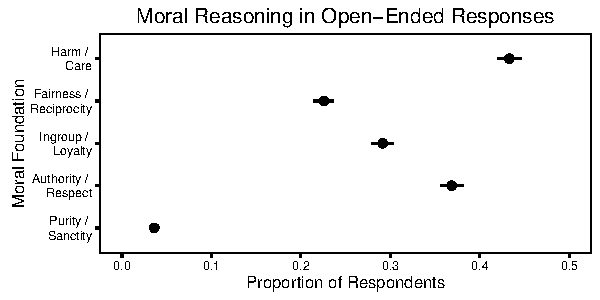
\includegraphics{../calc/fig/prop_mft.pdf}
\caption{Proportion of respondents mentioning each of the moral foundations in any of their open-ended responses, along with 95\% confidence intervals.}\label{fig:prop_ideol}
\end{figure}

The moral foundation most frequently mentioned is harm/care: About 40\% of the respondents mentioned at least one word included in respective dictionary. The second most frequently mentioned moral foundation is authority/respect with about 33\%. The proportion of respondents emphasizing ingroup/respect of fairness reciprocity is slightly lower with about 26\% and 20\%, respectively. Purity/sanctity, on the other hand, was almost never mentioned by any of the respondents. This finding is surprising, since other studies found the foundation to be an important predictor of divisive political attitudes \citep{koleva2012tracing}. This result suggests that the terms contained in the purity/sanctity dictionary might be too uncommon in the context of politics and therefore not relevant for attitude expression. Due to the very rare mentioning of the purity/sanctity dimension, the subsequent analyses will concentrate on the remaining four moral foundations.\footnote{Unfortunately, this issue cannot not be properly addressed by relying on tf-idf cosine scores. The weighting can correct for some distortions due to individual ubiquitous terms in the dictionaries, but it cannot compensate for the fact that the purity dictionary as a whole contains many words that are never mentioned by respondents.} Subsequent analyses focusing on the dimension of purity/sanctity in open-ended survey responses might necessitate a revision of the moral foundation dictionary.

Overall, Figure~\ref{fig:prop_ideol} shows that a substantial proportion of individuals evokes moral considerations when describing their political attitudes even when they are not explicitly asked about morality. However, we are ultimately interested in ideological differences in the emphasis of moral foundations in open-ended responses. As such, we now turn to a more in-depth analysis of the similarity scores as measures of moral reasoning.

We begin by estimating a set of Tobit regressions using ideology (and the control variables discussed above) to predict the individual similarity score for each of the moral foundations (excluding purity/sanctity).\footnote{The full estimates for this and all subsequent models discussed the remainder of the paper are presented in Appendix~\ref{app:tables}.} To reiterate, the similarity score measures the overlap between individual open-ended responses and the dictionaries for each foundation and has a value of 0 if none of the words in a dictionary appear in a response. Figure~\ref{fig:tobit_ideol} compares liberals and conservatives while holding all other variables constant at their respective means. The effects of ideology (liberal - conservative) estimated in the Tobit model are decomposed into two parts: the left panel displays the change in probability of the similarity score to be larger than zero (i.e. the probability of mentioning a specific foundation at all), whereas the right panel displays the expected change in the similarity score given that it is larger than zero (i.e. the degree of emphasis on a foundation given that it was mentioned, measured in standard deviations).

\begin{figure}[ht]\centering
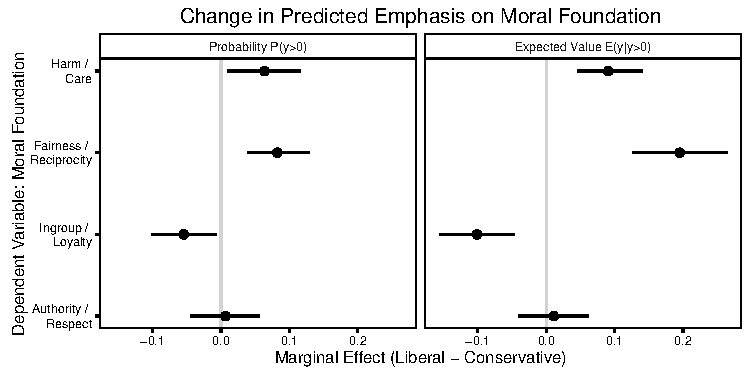
\includegraphics{../calc/fig/tobit_ideol.pdf}
\caption{Difference between liberals and conservatives in the probability of mentioning each moral foundation (left panel), and in the similarity score given that the foundation was mentioned (right panel), holding all other control variables at their respective means (along with 95\% confidence intervals). Positive values indicate that liberals are more likely to mention the respective foundation than conservatives (left panel), or emphasize it more than conservatives (right panel), and vice versa. Estimates are based on separate Tobit models for each foundation's similarity score. %Full model results are displayed in Table~\ref{tab:m2ideol}.
}\label{fig:tobit_ideol}
\end{figure}

Positive values denote a higher probability of mentioning the respective moral foundation (left panel) or a higher similarity score (right panel) of a response among individuals who identified as liberals, while negative values indicate a a higher probability/higher score among conservatives. The effects are consistent with the the expectations of MFT for three out of four moral foundations. Liberals are significantly more likely to mention the foundations of harm/care and fairness/reciprocity. For respondents who identified as liberal as compared to conservative, the probability of referencing these two foundations is increased by about 10\%. Furthermore, given that respondents mention these two foundations at all, liberals emphasize it more than conservatives when evaluating political parties and candidates. The similarity score for the harm/care foundation is about 0.1 standard deviations higher among liberals than conservatives. The effect is slightly larger for the fairness/reciprocity dimension. Conversely, being conservative increases the similarity score for the foundation of ingroup/loyalty by about 0.1 standard deviations. For the authority/respect dimension, we do not observe any significant differences between liberals and conservatives.

Taken together, the results are largely consistent with previous findings in the literature on MFT. Individuals evoke moral considerations when evaluating political parties and candidates without being explicitly asked about morality. Furthermore, there are systematic differences between liberals and conservatives in their reliance on binding and individualizing foundations \citep[see][for similar ideological differences when analyzing the content of life-narrative interviews]{mcadams2008family}. However, the fact that the authority/respect foundation showed insignificant patterns could suggest that the public's reliance on moral foundations may be more context-specific than previously thought.


\subsubsection{Consequences and Political Relevance of Moral Reasoning}

A skeptical reader might argue that ideological differences in moral reasoning are not unequivocally consistent with MFT because open-ended responses provide a less precise measure as compared to the MFQ. In order to alleviate this concern, We proceed to show that the expression of specific moral foundations in open-ended responses has important effects on political attitudes and behavior that match existing findings in the literature. Previous research relying on the MFQ has linked moral foundations to an array of political outcomes, such as candidate preferences \citep{iyer2010beyond} and voting behavior \citep{franks2015using}. Do we see the same patterns for explicit moral reasoning as compared to latent moral foundations?

\begin{figure}[ht]\centering
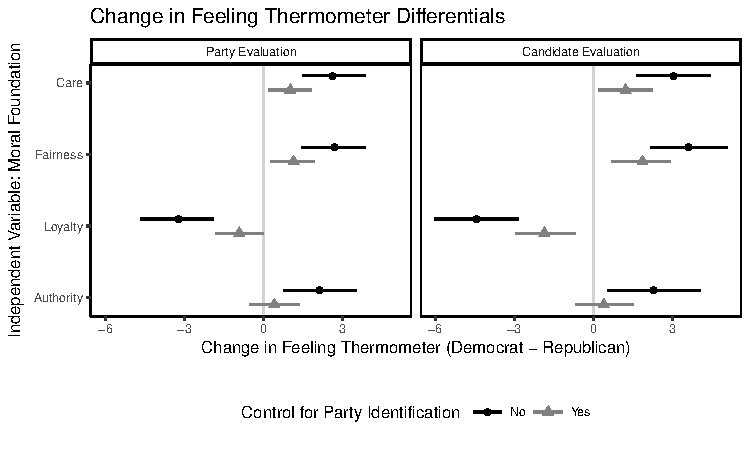
\includegraphics{../calc/fig/ols_feel.pdf}
\caption{Change in predicted feeling thermometer differential when similarity score is increased from its minimum (no overlap between dictionary and response) by one standard deviation, holding all other control variables constant at their respective means (along with 95\% confidence intervals). Positive values indicate that respondents who emphasized the respective foundation evaluated the Democratic candidate/party more favorably than the Republican candidate/party, and vice versa. Estimates are based on a single OLS model (using robust standard errors) including similarity scores for each foundation and gray triangles indicate estimates while additionally controlling for party identification. %Full model results are displayed in Table~\ref{tab:m7feel}.
}\label{fig:ols_feel}
\end{figure}

As a first step, we examine the relationship of moral reasoning and attitudes towards political parties and candidates. Figure~\ref{fig:ols_feel} presents OLS estimates where feeling thermometer differentials between the Republican and the Democratic party (left panel) and between both Presidential candidates (right panel) are regressed on similarity scores for all moral foundations (including the control variables discussed above). Positive values indicate more favorable evaluations for the Democratic candidate or party and negative values indicate more favorable evaluations of the Republican candidate or party. The patterns are largely consistent with the previous results on ideological differences. Individuals who emphasize considerations related to harm/care, and fairness/reciprocity evaluate the Democratic party/candidate on average about 5 points higher than the Republican party/candidate (on a 100 point scale). On the other hand, if individuals emphasized the ingroup/loyalty dimension, they reported stronger preferences for the Republican party/candidate. These effects are robust after controlling for individual party identification. Thus, in both analyses in Figure~\ref{fig:ols_feel}, we observed sizable and significant effects for the influence of moral reasoning.

\begin{figure}[ht]\centering
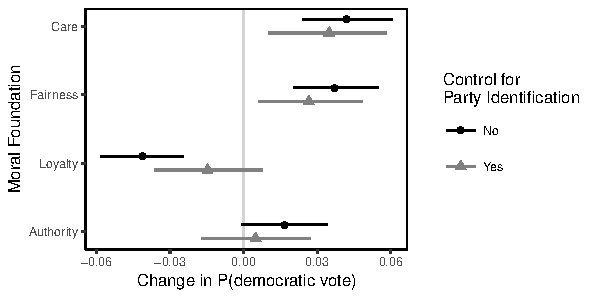
\includegraphics[scale=.9]{../calc/fig/logit_vote.pdf}
\caption{Change in predicted probabilities to vote for Democratic candidate when similarity score is increased from its minimum (no overlap between dictionary and response) by one standard deviation, holding all other control variables constant at their respective means (along with 95\% confidence intervals). Positive values indicate that respondents who emphasize the respective foundation are more likely to vote for the Democratic candidate, and vice versa. Estimates are based on a single logit model including similarity scores or each foundation and dotted lines indicate estimates while additionally controlling for party identification. %Full model results are displayed in Table~\ref{tab:m8vote}.
}\label{fig:logit_vote}
\end{figure}

Figure~\ref{fig:logit_vote} presents the changes in expected probabilities of voting for the Democratic (vs. the Republican) presidential candidate in the 2012 election for individuals emphasizing the moral foundations in their open-ended responses. The estimated probabilities are based on logit models including similarity scores for each moral foundation as independent variables (as well as  the remaining controls), which were held constant at their mean values when computing expected values. Again, the patterns are strikingly similar to the results presented thus far, and largely consistent with MFT. Individuals who emphasized moral considerations related to the harm/care and fairness/reciprocity foundations are more likely to vote for Barack Obama than for Mitt Romney. Respondents who emphasized the ingroup/loyalty foundation, on the other hand, were less likely to vote for Obama. 

The effects on political evaluations and vote choice might not seem large, but bear in mind that the measure of moral reasoning is solely based on open-ended responses, in which respondents were \textit{not} explicitly asked about morality. Nevertheless, the moral considerations evoked were powerfully related to party and candidate evaluations as well as vote choice, even after controlling for strength of party identification and the length of individual responses. Overall, the analyses show that people's open-ended comments about both candidates and both parties are imbued with moral content and that these comments relate to political judgments in the manner predicted by MFT.


\subsubsection{Determinants of Moral Reasoning}

Having shown that liberals and conservatives differ with regard to the moral foundations they emphasize when evaluating political actors and that these differences allow us to predict preferences and vote choice, we now investigate whether the reliance on moral considerations varies between individuals as a product of political knowledge and exposure to political discourse. Campaign exposure and discussions influence the degree to which political attitudes are moralized to the extent to which individuals adopt moral rhetoric from elites and their peers. As such, we first focus on determinants of the general tendency to emphasize \textit{any} moral foundation by regressing the sum of similarity scores for each individual on political knowledge, political media exposure, and frequency of political discussions. Figure~\ref{fig:tobit_learn} depicts the respective effects when each independent variable is increased from its empirical minimum value to its empirical maximum value, holding all other variables (including the logged number of words in each individual response) constant at their means. Again, estimates are based on tobit models that take into account the censoring of the moral reasoning measure and effects are decomposed into probability of mentioning any moral foundation (left panel) as well as the emphasis on morality, given that any foundation was mentioned (right panel).

\begin{figure}[h]\centering
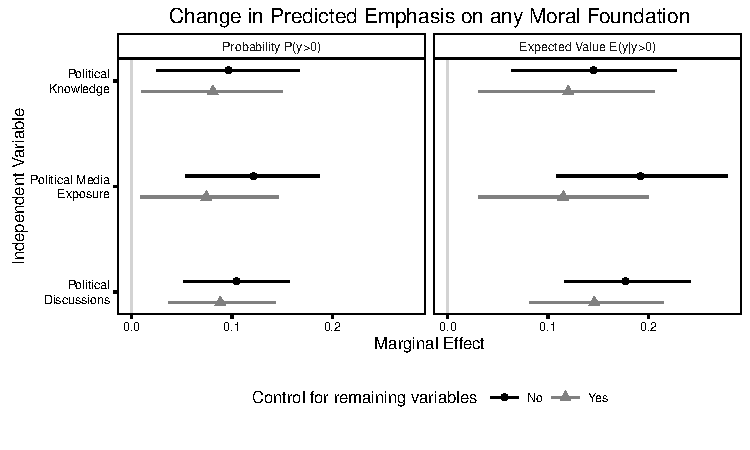
\includegraphics{../calc/fig/tobit_learn.pdf}
\caption{Change in predicted overall reliance on moral foundations depending on political knowledge, media exposure, and frequency of political discussions. The plot shows differences in predicted probabilities of mentioning any moral foundation (left panel) as well as in the summed similarity scores given that any foundation was mentioned (right panel), if each of the independent variables is increased from its minimum to its maximum value holding all other variables constant at their respective means (along with 95\% confidence intervals). Positive values indicate higher probability of mentioning, or stronger emphasis on moral foundations. Estimates are based on Tobit models and gray triangles indicate estimates while additionally controlling for the remaining variables presented in the figure. %Full model results are displayed in Table~\ref{tab:m3learn}.
}\label{fig:tobit_learn}
\end{figure}

All variables considered here have a positive effect on the individual likelihood to mention as well as the respective emphasis on moral foundations when evaluating political parties and candidates. Higher political knowledge, higher exposure to political media and news, as well as more frequent political discussions increase the degree to which individuals rely on moral considerations. Thus, citizens \textit{learn} to embed moral reasoning in their political evaluations. While moral intuitions themselves might well be innate, the extent to which individuals make use of these intuitions when thinking about politics and evaluating political actors is context-dependent and subject to individual heterogeneity.

The significant positive effect of frequent political discussions (even after controlling for the remaining variables, political knowledge and media exposure), is especially interesting in this context. Citizens, who engage in frequent political arguments are more likely to use moral considerations when evaluating candidates and parties. This result suggests that morality serves as a rhetorical tool utilized to convince others of certain political views.\footnote{This conclusion is also supported by the finding that the reliance on moral considerations is more pronounced among individuals who engage in non-conventional forms of participation (protests, signing petitions, wearing campaign buttons). On the other hand, simply participating in the previous election did not increase the emphasis of moral foundations significantly. These results are presented in the appendix, Figure~\ref{fig:tobit_learn_participation}.}

Beyond their effects on \textit{general} moral reasoning, we want to investigate whether the effects of political knowledge, media exposure, and discussions influence the systematic differences between liberals and conservatives in the emphasis on \textit{specific} dimensions. Consider again the results presented in Figure~\ref{fig:tobit_ideol}, which showed that liberals were more likely to emphasize the harm/care and fairness/reciprocity dimensions, while conservatives were more likely to emphasize the ingroup/loyalty foundation. In order to investigate whether the differences are conditional on political knowledge, media exposure, and discussions, we extend the original models by including interaction terms for each of the three variables that have been shown to influence the overall reliance on moral considerations. Based on these models, we can examine whether the same ideological pattern can be recovered for individuals with low or high levels of political knowledge, media exposure, and discussion frequency.

\begin{figure}[ht]\centering
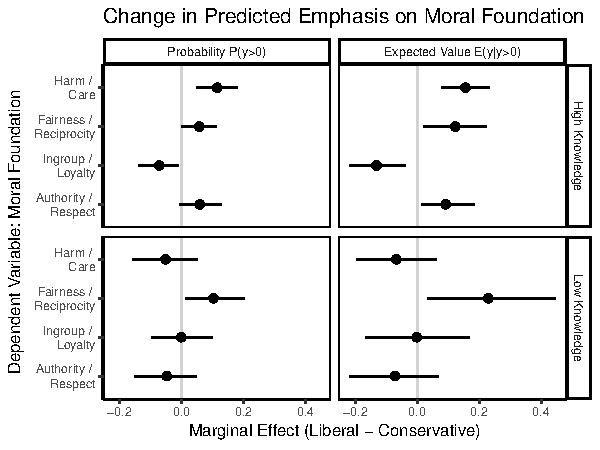
\includegraphics{../calc/fig/tobit_ideol_know.pdf}
\caption{Difference between liberals and conservatives in the probability of mentioning each moral foundation (left panel), and in the similarity score given that the foundation was mentioned (right panel), comparing individuals with low and high levels of political knowledge while holding all other control variables at their respective means (along with 95\% confidence intervals). Positive values indicate that liberals are more likely to mention the respective foundation than conservatives (left panel), or emphasize it more than conservatives (right panel), and vice versa. Estimates are based on separate Tobit models for each foundation's similarity score where ideology is interacted with political knowledge.}\label{fig:tobit_ideol_know}
\end{figure}

Figure~\ref{fig:tobit_ideol_know} displays the analyses equivalent to the previous results in Figure~\ref{fig:tobit_ideol}, now differentiating between individuals with high and low levels of political knowledge. While we can observe the same systematic differences between liberals and conservatives for individuals with high levels of political knowledge (upper panels), the effects of ideology disappear among individuals with low levels of political knowledge (lower panels) for all foundations except fairness/reciprocity. As such, we recover systematic differences in moral reasoning between liberals and conservatives only among the sub-group of highly knowledgeable respondents. It is worth noting again that all models presented here control for education and logged overall response length, which should account for potential confounding factors related to the respondents' eloquence when discussing their political attitudes.

\begin{figure}[ht]\centering
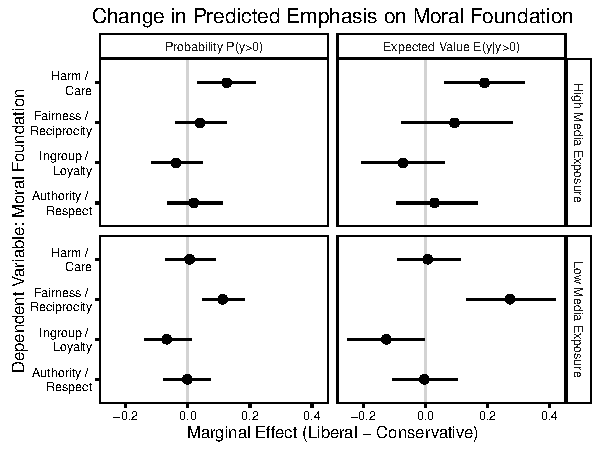
\includegraphics{../calc/fig/tobit_ideol_media.pdf}
\caption{Difference between liberals and conservatives in the probability of mentioning each moral foundation (left panel), and in the similarity score given that the foundation was mentioned (right panel), comparing individuals with low and high levels of political media exposure while holding all other control variables at their respective means (along with 95\% confidence intervals). Positive values indicate that liberals are more likely to mention the respective foundation than conservatives (left panel), or emphasize it more than conservatives (right panel), and vice versa. Estimates are based on separate Tobit models for each foundation's similarity score where ideology is interacted with political media exposure.}\label{fig:tobit_ideol_media}
\end{figure}

Next, we turn to a parallel analysis focusing on the influence of political media exposure instead of political knowledge. Figure~\ref{fig:tobit_ideol_media} compares the ideological differences for individuals with high and low levels of media exposure. Interestingly, the results look somewhat different than for political knowledge. While we again see that the higher emphasis on the harm/care foundation among liberals is only recovered among individuals who are frequent recipients of political news, the reverse is true for the fairness/reciprocity and ingroup/loyalty dimension. In both cases, the effects of ideology consistent with MFT only appear among individuals who are not frequently exposed to political news. This result is interesting since it suggests that media consumption can decrease the ideological divide in moral considerations expressed in politics.

\begin{figure}[ht]\centering
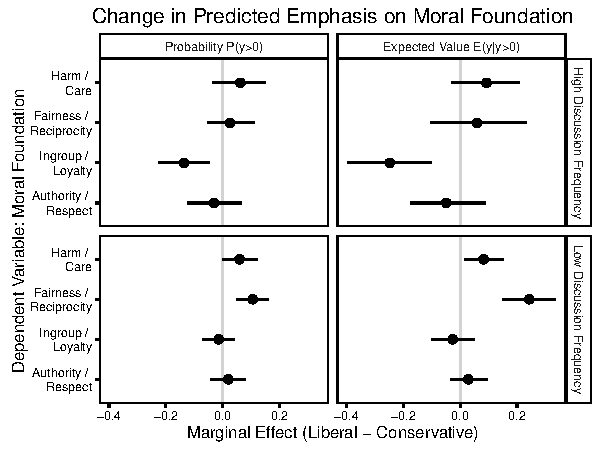
\includegraphics{../calc/fig/tobit_ideol_disc.pdf}
\caption{Difference between liberals and conservatives in the probability of mentioning each moral foundation (left panel), and in the similarity score given that the foundation was mentioned (right panel), comparing individuals with low and high levels of political discussions while holding all other control variables at their respective means (along with 95\% confidence intervals). Positive values indicate that liberals are more likely to mention the respective foundation than conservatives (left panel), or emphasize it more than conservatives (right panel), and vice versa. Estimates are based on separate Tobit models for each foundation's similarity score where ideology is interacted with political discussions.}\label{fig:tobit_ideol_disc}
\end{figure}

Lastly, Figure~\ref{fig:tobit_ideol_disc} differentiates between individuals who discuss politics more or less frequently. Again, the results are not as straightforward as in the case of political knowledge. There are significant differences in the reliance on the harm/care and fairness/reciprocity dimension between liberals and conservatives who do \textit{not} talk about politics with their peers, while no statistically significant effects are found among individuals who do discuss politics frequently. On the other hand, the ideological divide in the emphasis on the ingroup/loyalty foundation is only recovered among individuals who discuss politics frequently.

These results draw much more nuanced picture of the ideological differences in moral reasoning than previous studies. The patterns are only unequivocally consistent with MFT among politically knowledgeable respondents.\footnote{This is especially noteworthy given that many studies on MFT are based on opt-in samples collected through \url{www.yourmorals.org}, which potentially leads to biases towards higher education among respondents.} However, the picture is more complicated when looking at the influence of media exposure and political discussions. Exposure to political discourse increases the ideological divide on some dimensions but decreases it on others. Explaining these patterns requires a more detailed analyses of the content of the media coverage as well as the nature of political discussions. For now, we leave this issue as a fruitful area for future research efforts.

Furthermore, it should be emphasized that not all changes discussed in Figures~\ref{fig:tobit_ideol_know} through \ref{fig:tobit_ideol_disc} are necessarily statistically significant \citep[c.f.,][]{gelman2006difference}.\footnote{See the appendix, Figure~\ref{fig:tobit_ideol_difdif} for detailed results on the statistical significance of the difference-in-differences between the comparisons.} Nevertheless, we can conclude from the analyses that whether researchers are able to recover systematic ideological differences in moral reasoning consistent with MFT is highly conditional on individual-level factors. Overall, political knowledge, media exposure and discussion frequency not only affect general levels of moral reasoning but also moderate the ideological gap between liberals and conservatives. Some portion of the ideological differences in emphasis on moral foundations can therefore be described as a product of learning in the political environment. However, the nature of the relationship between the political context and individual moral reasoning is complex and requires further investigation.


\section{Conclusion}

There is much more to be learned about the relationship between moral foundations and broader political attitudes and ideology \citep[e.g.,][]{feldman2013political}. To fully understand how political views are rooted in morality, researchers need to take a closer look at the conditions under which citizens express moral considerations in the context of politics. In contrast to previous accounts of MFT, we argue that the reliance on moral reasoning is moderated by political knowledge, media exposure, and political discussions. Not every individual necessarily thinks about politics in terms of morality. Rooting political preferences in deeper moral foundations requires exposure to a political discourse that fosters such a connection \citep[c.f.,][]{clifford2015concerns}.

This study utilized open-ended survey responses to investigate the conditionality of MFT in political reasoning. The analyses of open-ended survey responses is valuable in this context because it allows us to evaluate whether citizens make references to moral considerations in a political context that does not induce an explicit connection to morality. As such, we can directly investigate when and how ideological differences in the emphasis of moral foundations manifest themselves in individual reasoning about political actors. More generally, open-ended survey responses provide a promising and still largely neglected data source to investigate the determinants and structure of ideology and political reasoning. In particular, scholars can directly assess moral reasoning in surveys that do not contain the MFQ or related measures, simply by relying on open-ended survey responses.

The empirical analyses presented here extend and qualify previous research on moral foundations and ideology. We found systematic patterns in the emphasis on moral considerations among liberals and conservatives consistent with MFT for three out of four foundations. Liberals are more likely to mention considerations related to harm/care and fairness/reciprocity when discussing their political preferences, whereas conservatives are more likely to emphasize the moral foundation of ingroup/loyalty. The second part of the analyses focused on the political relevance of moral reasoning as conceptualized by open-ended survey responses. Here, the results revealed consistent relationships between individual moral foundations and political preferences or voting behavior, which showed that moral reasoning (measured via open-ended survey responses) is a politically meaningful and influential concept. Lastly, political knowledge and exposure to political discourse increase the reliance on moral considerations. The evidence suggests that moral reasoning in political judgment is conditional on multiple individual-level factors and therefore likely to be part of a broader political learning process. At least in some cases, this learning process appears to imply an increased differentiation between liberals and conservatives in terms of the focus on specific foundations as described by MFT.

Moral foundations can provide a powerful source of structure in political belief systems. However, we cannot assume that the link between morality and politics is homogeneous across individuals and contexts. The present study therefore reaffirms the importance of moral reasoning in politics but highlights its conditionality. The results clarify instances when moral foundations are indeed influential in shaping ideological differences. Individual-level factors such as political knowledge, media exposure, and discussion frequency determine whether and how liberals and conservatives evoke moral considerations in political judgment. Ultimately, a deeper understanding of their influence necessitates further analyses of the broader political context that shapes individual information environments. As such, future research could examine how the endorsement of moral foundations varies over time and across campaigns. Such an investigation would allow us to further illuminate how exposure to political discourse fosters ideological differences in moral reasoning. A better understanding of the antecedents of this ideological divide is especially important in times of growing partisan polarization.

\clearpage
\bibliographystyle{/data/Dropbox/Uni/Lit/apsr2006}
\bibliography{/data/Dropbox/Uni/Lit/Literature}

\clearpage
\footnotesize\singlespacing
\appendices
\appendixpage
\renewcommand\thesubsection{\Roman{subsection}}
\begin{flushleft}
Kraft, Patrick W. 2016.\\``Moral Foundations of Political Reasoning. Investigating the Moral Underpinnings of Political Judgment.''

\startcontents[sections]
\printcontents[sections]{l}{1}{\setcounter{tocdepth}{2}}
\clearpage

\section{Moral Foundations Dictionary}\label{app:dict}
\renewcommand\thefigure{\thesection.\arabic{figure}}
\renewcommand\thetable{\thesection.\arabic{table}}
\setcounter{figure}{0}
\setcounter{table}{0}

\textit{Sources:}\\
\citet{graham2009liberals}, as well as \url{http://www.moralfoundations.org/}
\vspace{.5cm}

\textit{Note:}\\
Words with (*) indicate that the word stem rather than the exact word was matched in the open-ended survey responses.
\vspace{.5cm}

\textbf{Harm:}\\
safe*, peace*, compassion*, empath*, sympath*, care, caring, protect*, shield, shelter, amity, secur*, benefit*, defen*, guard*, preserve, harm*, suffer*, war, wars, warl*, warring, fight*, violen*, hurt*, kill, kills, killer*, killed, killing, endanger*, cruel*, brutal*, abuse*, damag*, ruin*, ravage, detriment*, crush*, attack*, annihilate*, destroy, stomp, abandon*, spurn, impair, exploit, exploits, exploited, exploiting, wound*
\vspace{.5cm}

\textbf{Fairness:}\\
fair, fairly, fairness, fair*, fairmind*, fairplay, equal*, justice, justness, justifi*, reciproc*, impartial*, egalitar*, rights, equity, evenness, equivalent, unbias*, tolerant, equable, balance*, homologous, unprejudice*, reasonable, constant, honest*, unfair*, unequal*, bias*, unjust*, injust*, bigot*, discriminat*, disproportion*, inequitable, prejud*, dishonest, unscrupulous, dissociate, preference, favoritism, segregat*, exclusion, exclud*
\vspace{.5cm}

\textbf{Ingroup:}\\
together, nation*, homeland*, family, families, familial, group, loyal*, patriot*, communal, commune*, communit*, communis*, comrad*, cadre, collectiv*, joint, unison, unite*, fellow*, guild, solidarity, devot*, member, cliqu*, cohort, ally, insider, foreign*, enem*, betray*, treason*, traitor*, treacher*, disloyal*, individual*, apostasy, apostate, deserted, deserter*, deserting, deceiv*, jilt*, imposter, miscreant, spy, sequester, renegade, terroris*, immigra*
\vspace{.5cm}

\textbf{Authority:}\\
obey*, obedien*, duty, law, lawful*, legal*, duti*, honor*, respect, respectful*, respected, respects, order*, father*, mother, motherl*, mothering, mothers, tradition*, hierarch*, authorit*, permit, permission, status*, rank*, leader*, class, bourgeoisie, caste*, position, complian*, command, supremacy, control, submi*, allegian*, serve, abide, defere*, defer, revere*, venerat*, comply, defian*, rebel*, dissent*, subver*, disrespect*, disobe*, sediti*, agitat*, insubordinat*, illegal*, lawless*, insurgent, mutinous, defy*, dissident, unfaithful, alienate, defector, heretic*, nonconformist, oppose, protest, refuse, denounce, remonstrate, riot*, obstruct
\vspace{.5cm}

\textbf{Purity:}\\
piety, pious, purity, pure*, clean*, steril*, sacred*, chast*, holy, holiness, saint*, wholesome*, celiba*, abstention, virgin, virgins, virginity, virginal, austerity, integrity, modesty, abstinen*, abstemiousness, upright, limpid, unadulterated, maiden, virtuous, refined, intemperate, decen*, immaculate, innocent, pristine, humble, disgust*, deprav*, disease*, unclean*, contagio*, indecen*, sin, sinful*, sinner*, sins, sinned, sinning, slut*, whore, dirt*, impiety, impious, profan*, gross, repuls*, sick*, promiscu*, lewd*, adulter*, debauche*, defile*, tramp, prostitut*, unchaste, wanton, profligate, filth*, trashy, obscen*, lax, taint*, stain*, tarnish*, debase*, desecrat*, wicked*, blemish, exploitat*, pervert, wretched*
\vspace{.5cm}

%\textbf{General:}\\
%righteous*, moral*, ethic*, value*, upstanding, good, goodness, principle*, blameless, exemplary, lesson, canon, doctrine, noble, worth*, ideal*, praiseworthy, commendable, character, proper, laudable, correct, wrong*, evil, immoral*, bad, offend*, offensive*, transgress*, honest*, lawful*, legal*, piety, pious, wholesome*, integrity, upright, decen*, indecen*, wicked*, wretched*

\end{flushleft}

\clearpage
\section{Additional Descriptive Information}\label{app:oview}
\renewcommand\thefigure{\thesection.\arabic{figure}}
\renewcommand\thetable{\thesection.\arabic{table}}
\setcounter{figure}{0}
\setcounter{table}{0}

% latex table generated in R 3.3.0 by xtable 1.8-2 package
% Fri Sep  2 15:41:09 2016
\begin{table}[ht]
\centering
\begin{tabular}{lcc}
  \hline
 & N & Percent \\ 
  \hline
Spanish Interview & 228 & 3.86 \\ 
  No Responses & 417 & 7.05 \\ 
   \hline
\end{tabular}
\caption{Missing open-ended responses} 
\label{tab:app_mis}
\end{table}


\begin{figure}[h]\centering
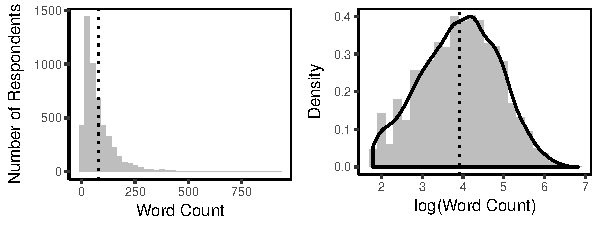
\includegraphics[width=\textwidth]{../calc/fig/app_wc.pdf}
\caption{Histograms displaying the distribution of individual response lengths in number of words for each respective item category. Dotted lines indicate the average response length.}\label{fig:appB2num}
\end{figure}

\begin{figure}[h]\centering
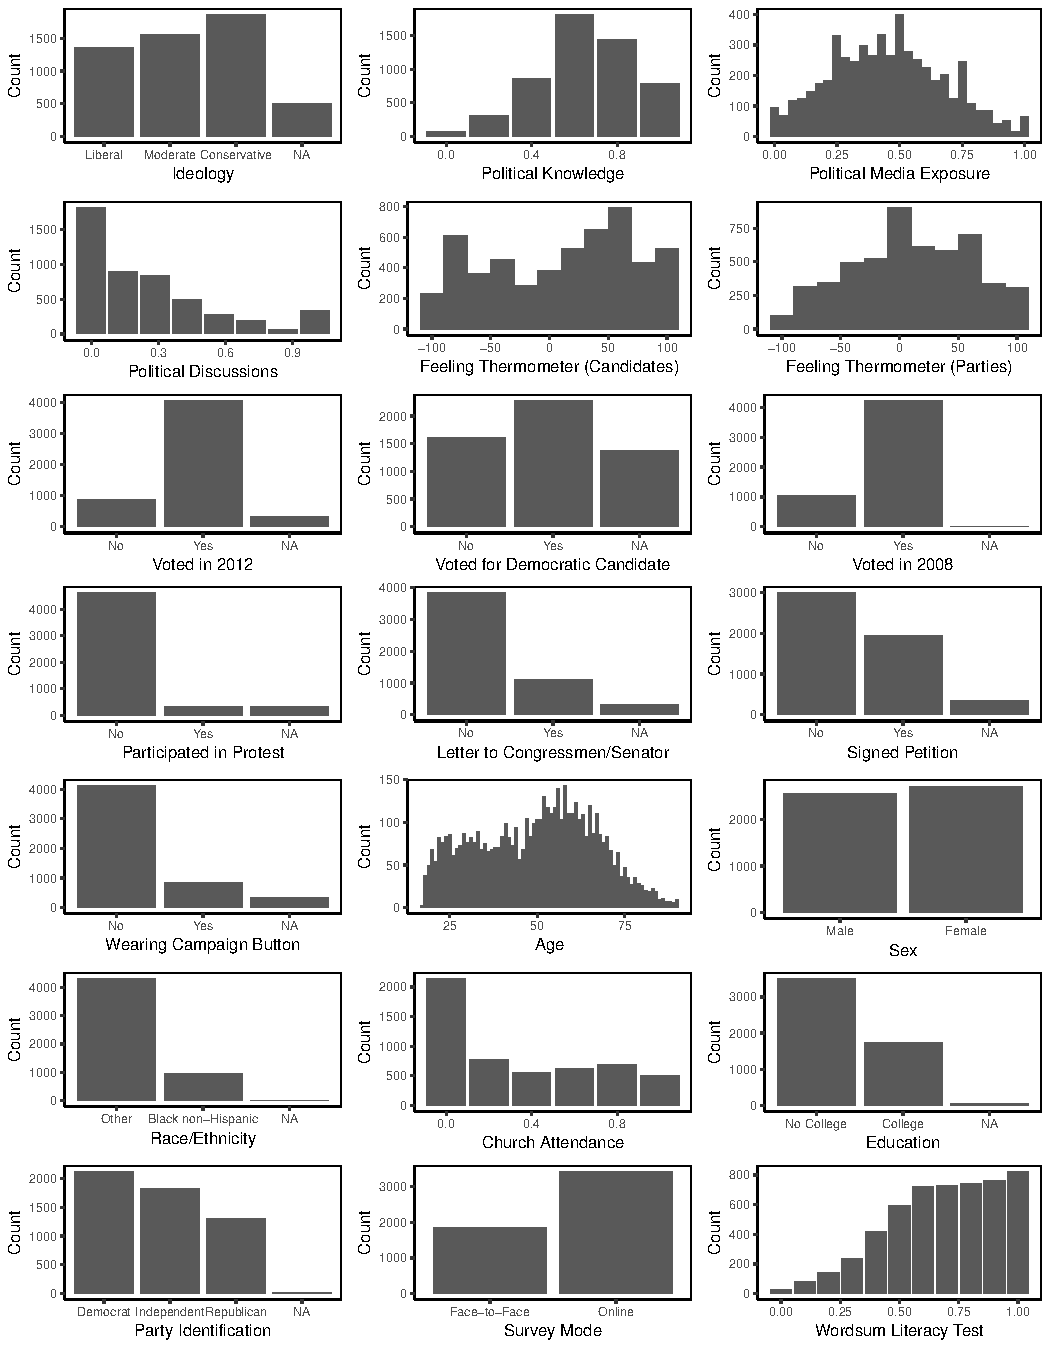
\includegraphics[width=\textwidth]{../calc/fig/app_desc.pdf}
\caption{Histograms for variables included in analyses.}\label{fig:app_desc}
\end{figure}

\clearpage
\section{Description of Moral Reasoning Measure}\label{app:measure}

This part of the appendix contains a detailed description of the measure of moral reasoning used throughout the paper. It is based on open-ended survey responses as well as the moral dictionary proposed by \citet{graham2009liberals}. All techniques described here are adapted from common approaches in quantitative text analysis and information retrieval \citep[see for exampe][for an introduction and from which much of the notation in this part of the appendix is adapted]{manning2008introduction}.

As a first step, each individual response as well as the moral foundations dictionaries are converted into a \textit{document-term matrix}. Each row in the document-term matrix represents one document (i.e. the collection of open-ended responses for one individual, or the dictionary for a single moral foundation, respectively). Each column represents a term that is contained in the complete vocabulary of the corpus (i.e. all columns encompass the set of unique words contained in all documents). Each element in the matrix indicates the number of times the term is included in the respective document. As such, the matrix consists of raw frequencies of term $t$ in document $d$ (often denoted by tf$_{t,d}$).

However, in the context of information retrieval that aims at matching string queries with most relevant matches out of a set of documents, term frequencies are usually weighted by the \textit{inverse document frequency} in order to account for the fact that some terms have more discriminative power than others. The underlying logic is that a word that appears in almost all of the documents should be less decisive in affecting the similarity between the query and the document than a term that only appears in a selection of documents. The inverse document frequency is usually defined as
\begin{equation}
\text{idf}_t = \log \tfrac{N}{\text{df}_t},
\end{equation}
where $N$ is the total number of documents in the corpus, and $df_t$ denotes the number of documents in which term $t$ occurs. The tf-idf score of term $t$ in document $d$ is then computed as
\begin{equation}
\text{tf-idf}_{t,d} = \text{tf}_{t,d} * \text{idf}_t.
\end{equation}
Raw term frequencies are therefore weighted by the inverse of the term's document frequency, which leads to increased (decreased) values if a term is only included in few (many) documents. We can now represent each moral dictionary and response as a vector of tf-idf scores for each term. For convenience, let $w_{t,d}$ be the tf-idf score for term $t$ in the dictionary and document $d$ (which could be a moral dictionary or an open-ended response). Then,
\begin{align}
\vec{m}_j &= \left(w_{1,j},w_{2,j},\cdots, w_{T,j}\right) \\
\vec{r}_n &= \left(w_{1,n},w_{2,n},\cdots, w_{T,n}\right),
\end{align}
where $\vec{m}_j$ denotes the moral dictionary for foundation $j\in\{1,\cdots,J\}$, $\vec{r}_n$ denotes the open-ended responses of individual $n\in\{1,\cdots,N\}$, and $T$ denotes the total number of unique terms in the entire text corpus. This representation of documents and queries (or in our case dictionaries) is usually described as the \textit{vector space model} for representing the corpus.

Each moral dictionary and open-ended response is now represented as a vector of length $T$. A common measure of relevance, for example of a document ($\vec{r}_n$) for a keyword search query (in our case $\vec{m}_j$), is the cosine similarity:
\begin{equation}
\cos\theta_{j,n}=\dfrac{\vec{m}(j)\cdotp\vec{r}(n)}{|\vec{m}(j)||\vec{r}(n)|},
\end{equation}
where $\vec{m}(j)\cdotp\vec{r}(n)$ is the dot-product of the dictionary and the response, and $|\vec{m}(j)||\vec{r}(n)|$ is the product of the Euclidean norm of both vectors. $\theta_{j,n}$ can therefore be understood as the angle between the vector space representation of the moral foundation dictionary $j$ and the open-ended response of individual $n$. The cosine score is 1 if the relative frequency of words used by the respondent overlap completely with the terms in the dictionary (not that this holds irrespective of the length of the response), and 0 if there is no overlap.

\clearpage
\section{Additional Model Results and Robustness Checks}\label{app:robust}
\renewcommand\thefigure{\thesection.\arabic{figure}}
\renewcommand\thetable{\thesection.\arabic{table}}
\setcounter{figure}{0}
\setcounter{table}{0}


\begin{figure}[h]\centering
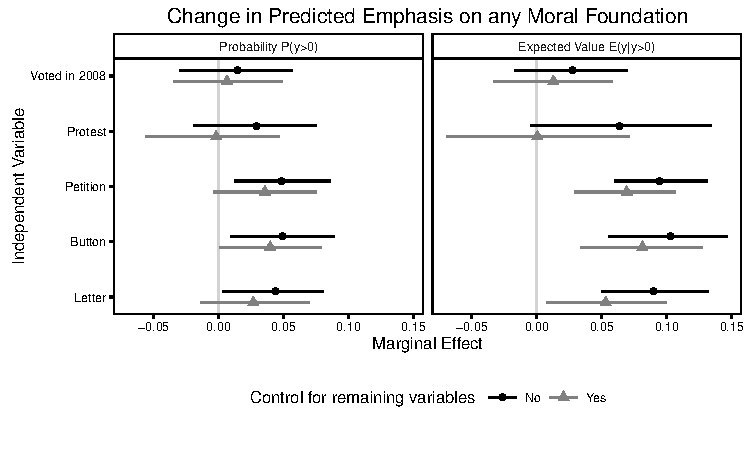
\includegraphics{../calc/fig/tobit_learn_participation.pdf}
\caption{Change in predicted overall reliance on moral foundations depending on previous turnout and non-conventional forms of participation (protest, petitions, campaign buttons). The plot shows differences in predicted probabilities of mentioning any moral foundation (left panel) as well as in the summed similarity scores given that any foundation was mentioned (right panel), if each of the independent variables is increased from its minimum to its maximum value holding all other variables constant at their respective means (along with 95\% confidence intervals). Positive values indicate higher probability of mentioning, or stronger emphasis on moral foundations. Estimates are based on Tobit models and gray triangles indicate estimates while additionally controlling for the remaining variables presented in the figure. %Full model results are displayed in Table~\ref{tab:m3learn}.
}\label{fig:tobit_learn_participation}
\end{figure}


\begin{figure}[ht]\centering
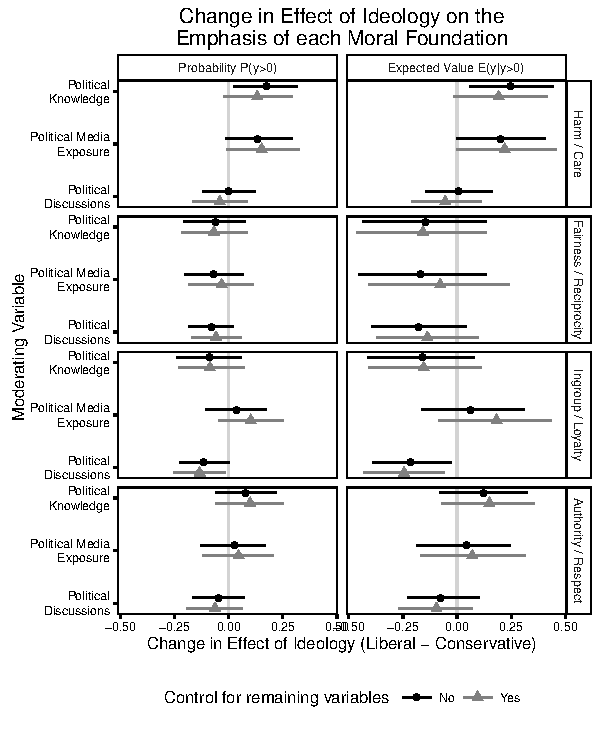
\includegraphics[scale=.8]{../calc/fig/tobit_ideol_difdif.pdf}
\caption{Change in effect of ideology on emphasis of each moral foundation moderated by political knowledge, media exposure, and frequency of political discussions (difference-in-difference). The plot shows how the difference between liberals and conservatives in predicted probabilities to mention each moral foundation, as well as the respective similarity scores, change if each of the independent variables is increased from its minimum to its maximum value holding all other variables constant at their respective means (along with 95\% confidence intervals). Positive values indicate that liberals are more likely to mention a specific moral foundation if they score high on the moderating variable (knowledge, exposure, discussions, previous turnout, protest behavior), and vice versa. Estimates are based on individual Tobit models for each foundation and gray triangles indicate estimates while controlling for all remaining variables displayed in the figure. %Full model results are displayed in Tables~\ref{tab:m4ideolearn2012a} to \ref{tab:tobit_learnideol}.
}\label{fig:tobit_ideol_difdif}
\end{figure}


\clearpage
\section{Tables of Model Estimates}\label{app:tables}
\renewcommand\thefigure{\thesection.\arabic{figure}}
\renewcommand\thetable{\thesection.\arabic{table}}
\setcounter{figure}{0}
\setcounter{table}{0}


%\subsection{Ideological differences in moral reasoning including 2008 ANES data}
%
%
% Table created by stargazer v.5.2 by Marek Hlavac, Harvard University. E-mail: hlavac at fas.harvard.edu
% Date and time: Wed, Jan 20, 2016 - 12:21:34 PM
% Requires LaTeX packages: dcolumn 
\begin{table}[ht] \centering 
  \caption{Logit Models Predicting References to four Moral Foundations using Ideology} 
  \label{tab:m2ideol} 
\tiny 
\begin{tabular}{@{\extracolsep{-15pt}}lD{.}{.}{-3} D{.}{.}{-3} D{.}{.}{-3} D{.}{.}{-3} D{.}{.}{-3} D{.}{.}{-3} D{.}{.}{-3} D{.}{.}{-3} } 
\\[-1.8ex]\hline 
\hline \\[-1.8ex] 
 & \multicolumn{8}{c}{\textit{Dependent variable:}} \\ 
\cline{2-9} 
\\[-1.8ex] & \multicolumn{2}{c}{Harm / Care} & \multicolumn{2}{c}{Fairness / Reciprocity} & \multicolumn{2}{c}{Ingroup / Loyalty} & \multicolumn{2}{c}{Authority / Respect} \\ 
 & \multicolumn{1}{c}{2012} & \multicolumn{1}{c}{2008} & \multicolumn{1}{c}{2012} & \multicolumn{1}{c}{2008} & \multicolumn{1}{c}{2012} & \multicolumn{1}{c}{2008} & \multicolumn{1}{c}{2012} & \multicolumn{1}{c}{2008} \\ 
\hline \\[-1.8ex] 
 Conservative & -0.340^{***} & -0.103 & -0.492^{***} & 0.019 & 0.298^{***} & 0.475^{***} & -0.272^{***} & -0.270^{*} \\ 
  & (0.083) & (0.148) & (0.092) & (0.191) & (0.090) & (0.171) & (0.085) & (0.152) \\ 
  Moderate & -0.338^{***} & -0.131 & -0.518^{***} & -0.273 & -0.026 & 0.367^{**} & -0.133 & -0.375^{**} \\ 
  & (0.084) & (0.150) & (0.094) & (0.209) & (0.095) & (0.178) & (0.085) & (0.159) \\ 
  Church Attendance & -0.016 & -0.039 & -0.0003 & -0.016 & 0.042^{**} & -0.012 & -0.030 & 0.052 \\ 
  & (0.019) & (0.035) & (0.022) & (0.046) & (0.021) & (0.039) & (0.020) & (0.036) \\ 
  Education (College Degree) & -0.017 & 0.139 & 0.322^{***} & 0.225 & 0.394^{***} & 0.554^{***} & 0.211^{***} & 0.321^{**} \\ 
  & (0.070) & (0.124) & (0.076) & (0.173) & (0.073) & (0.148) & (0.070) & (0.134) \\ 
  Age & -0.004^{*} & -0.015^{***} & 0.004^{*} & 0.011^{**} & -0.002 & -0.009^{**} & 0.007^{***} & -0.004 \\ 
  & (0.002) & (0.004) & (0.002) & (0.005) & (0.002) & (0.004) & (0.002) & (0.004) \\ 
  Sex (Female) & 0.200^{***} & 0.017 & 0.110 & 0.028 & -0.128^{*} & -0.432^{***} & -0.083 & -0.205^{*} \\ 
  & (0.066) & (0.118) & (0.074) & (0.157) & (0.072) & (0.134) & (0.067) & (0.124) \\ 
  Race (African American) & -0.017 & -0.066 & -0.103 & -0.042 & -0.189^{*} & -0.253 & 0.378^{***} & -0.081 \\ 
  & (0.091) & (0.150) & (0.105) & (0.207) & (0.103) & (0.180) & (0.091) & (0.160) \\ 
  Number of Words & 0.014^{***} & 0.017^{***} & 0.009^{***} & 0.008^{***} & 0.013^{***} & 0.015^{***} & 0.013^{***} & 0.011^{***} \\ 
  & (0.001) & (0.001) & (0.0005) & (0.001) & (0.001) & (0.001) & (0.001) & (0.001) \\ 
  Constant & -0.978^{***} & -0.614^{***} & -1.909^{***} & -3.026^{***} & -2.004^{***} & -2.071^{***} & -1.727^{***} & -1.366^{***} \\ 
  & (0.125) & (0.227) & (0.142) & (0.321) & (0.140) & (0.270) & (0.131) & (0.241) \\ 
 \hline \\[-1.8ex] 
Observations & \multicolumn{1}{c}{4,691} & \multicolumn{1}{c}{1,468} & \multicolumn{1}{c}{4,691} & \multicolumn{1}{c}{1,468} & \multicolumn{1}{c}{4,691} & \multicolumn{1}{c}{1,468} & \multicolumn{1}{c}{4,691} & \multicolumn{1}{c}{1,468} \\ 
Log Likelihood & \multicolumn{1}{c}{-2,765.763} & \multicolumn{1}{c}{-862.824} & \multicolumn{1}{c}{-2,310.347} & \multicolumn{1}{c}{-560.633} & \multicolumn{1}{c}{-2,440.218} & \multicolumn{1}{c}{-710.658} & \multicolumn{1}{c}{-2,702.758} & \multicolumn{1}{c}{-806.005} \\ 
Akaike Inf. Crit. & \multicolumn{1}{c}{5,549.527} & \multicolumn{1}{c}{1,743.648} & \multicolumn{1}{c}{4,638.693} & \multicolumn{1}{c}{1,139.266} & \multicolumn{1}{c}{4,898.436} & \multicolumn{1}{c}{1,439.317} & \multicolumn{1}{c}{5,423.517} & \multicolumn{1}{c}{1,630.010} \\ 
\hline 
\hline \\[-1.8ex] 
\textit{Note:}  & \multicolumn{8}{r}{$^{*}$p$<$0.1; $^{**}$p$<$0.05; $^{***}$p$<$0.01} \\ 
\end{tabular} 
\end{table} 

%
%\clearpage
%\subsection{Determinants of moral reasoning including 2008 ANES data}
%
%
% Table created by stargazer v.5.2 by Marek Hlavac, Harvard University. E-mail: hlavac at fas.harvard.edu
% Date and time: Sat, Jan 23, 2016 - 02:23:18 PM
% Requires LaTeX packages: dcolumn 
\begin{table}[ht] \centering 
  \caption{Logit models predicting overall references to any moral foundation} 
  \label{tab:m3learn} 
\tiny 
\begin{tabular}{@{\extracolsep{-15pt}}lD{.}{.}{-3} D{.}{.}{-3} D{.}{.}{-3} D{.}{.}{-3} D{.}{.}{-3} D{.}{.}{-3} D{.}{.}{-3} D{.}{.}{-3} } 
\\[-1.8ex]\hline 
\hline \\[-1.8ex] 
 & \multicolumn{8}{c}{\textit{Dependent variable:}} \\ 
\cline{2-9} 
\\[-1.8ex] & \multicolumn{8}{c}{Reference to any Moral Foundation} \\ 
 & \multicolumn{4}{c}{2012} & \multicolumn{4}{c}{2008} \\ 
\hline \\[-1.8ex] 
 Political Knowledge & 0.128^{***} &  &  & 0.130^{***} & 0.298^{**} &  &  & 0.282^{**} \\ 
  & (0.035) &  &  & (0.036) & (0.120) &  &  & (0.130) \\ 
  Political Media Exposure &  & 0.018^{***} &  & 0.010 &  & 0.017^{*} &  & -0.0003 \\ 
  &  & (0.006) &  & (0.006) &  & (0.010) &  & (0.011) \\ 
  Political Discussion &  &  & 0.097^{***} & 0.083^{***} &  &  & -0.012 & -0.018 \\ 
  &  &  & (0.020) & (0.021) &  &  & (0.027) & (0.028) \\ 
  Church Attendance & -0.019 & -0.018 & -0.018 & -0.020 & -0.037 & -0.043 & -0.056 & -0.056 \\ 
  & (0.020) & (0.020) & (0.021) & (0.021) & (0.033) & (0.032) & (0.035) & (0.035) \\ 
  Education (College Degree) & 0.282^{***} & 0.318^{***} & 0.375^{***} & 0.292^{***} & 0.305^{***} & 0.417^{***} & 0.429^{***} & 0.367^{***} \\ 
  & (0.082) & (0.080) & (0.083) & (0.087) & (0.118) & (0.110) & (0.123) & (0.127) \\ 
  Age & -0.001 & -0.002 & 0.001 & -0.002 & -0.009^{***} & -0.010^{***} & -0.007^{*} & -0.007^{*} \\ 
  & (0.002) & (0.002) & (0.002) & (0.002) & (0.003) & (0.003) & (0.004) & (0.004) \\ 
  Sex (Female) & 0.175^{**} & 0.153^{**} & 0.162^{**} & 0.207^{***} & -0.207^{*} & -0.171 & -0.229^{*} & -0.221^{*} \\ 
  & (0.071) & (0.070) & (0.073) & (0.075) & (0.114) & (0.108) & (0.121) & (0.122) \\ 
  Race (African American) & 0.358^{***} & 0.294^{***} & 0.294^{***} & 0.352^{***} & -0.084 & -0.114 & -0.058 & -0.002 \\ 
  & (0.096) & (0.093) & (0.097) & (0.100) & (0.132) & (0.122) & (0.140) & (0.143) \\ 
  Number of Words & 0.032^{***} & 0.032^{***} & 0.031^{***} & 0.031^{***} & 0.036^{***} & 0.036^{***} & 0.037^{***} & 0.036^{***} \\ 
  & (0.001) & (0.001) & (0.001) & (0.001) & (0.002) & (0.002) & (0.003) & (0.003) \\ 
  Constant & -1.239^{***} & -1.027^{***} & -1.062^{***} & -1.414^{***} & -0.734^{***} & -0.783^{***} & -0.617^{***} & -0.735^{***} \\ 
  & (0.150) & (0.129) & (0.131) & (0.159) & (0.203) & (0.196) & (0.216) & (0.234) \\ 
 \hline \\[-1.8ex] 
Observations & \multicolumn{1}{c}{5,147} & \multicolumn{1}{c}{5,177} & \multicolumn{1}{c}{4,842} & \multicolumn{1}{c}{4,807} & \multicolumn{1}{c}{1,845} & \multicolumn{1}{c}{2,031} & \multicolumn{1}{c}{1,648} & \multicolumn{1}{c}{1,646} \\ 
Log Likelihood & \multicolumn{1}{c}{-2,421.529} & \multicolumn{1}{c}{-2,437.572} & \multicolumn{1}{c}{-2,254.166} & \multicolumn{1}{c}{-2,231.179} & \multicolumn{1}{c}{-940.477} & \multicolumn{1}{c}{-1,044.857} & \multicolumn{1}{c}{-826.849} & \multicolumn{1}{c}{-823.971} \\ 
Akaike Inf. Crit. & \multicolumn{1}{c}{4,859.058} & \multicolumn{1}{c}{4,891.144} & \multicolumn{1}{c}{4,524.331} & \multicolumn{1}{c}{4,482.357} & \multicolumn{1}{c}{1,896.955} & \multicolumn{1}{c}{2,105.713} & \multicolumn{1}{c}{1,669.698} & \multicolumn{1}{c}{1,667.943} \\ 
\hline 
\hline \\[-1.8ex] 
\textit{Note:}  & \multicolumn{8}{r}{$^{*}$p$<$0.1; $^{**}$p$<$0.05; $^{***}$p$<$0.01} \\ 
\end{tabular} 
\end{table} 

%
% Table created by stargazer v.5.2 by Marek Hlavac, Harvard University. E-mail: hlavac at fas.harvard.edu
% Date and time: Wed, Jan 20, 2016 - 12:21:57 PM
% Requires LaTeX packages: dcolumn 
\begin{table}[ht] \centering 
  \caption{Logit Models Predicting References to Specific Moral Foundations (2012)} 
  \label{tab:m4ideolearn2012a} 
\tiny 
\begin{tabular}{@{\extracolsep{-15pt}}lD{.}{.}{-3} D{.}{.}{-3} D{.}{.}{-3} D{.}{.}{-3} D{.}{.}{-3} D{.}{.}{-3} D{.}{.}{-3} D{.}{.}{-3} } 
\\[-1.8ex]\hline 
\hline \\[-1.8ex] 
 & \multicolumn{8}{c}{\textit{Dependent variable:}} \\ 
\cline{2-9} 
\\[-1.8ex] & \multicolumn{4}{c}{Harm / Care} & \multicolumn{4}{c}{Fairness / Reciprocity} \\ 
\hline \\[-1.8ex] 
 Moderate & -0.285^{***} & -0.328^{***} & -0.361^{***} & -0.307^{***} & -0.513^{***} & -0.512^{***} & -0.493^{***} & -0.489^{***} \\ 
  & (0.085) & (0.084) & (0.087) & (0.089) & (0.096) & (0.095) & (0.098) & (0.100) \\ 
  Conservative & -0.281^{***} & -0.326^{***} & -0.371^{***} & -0.310^{***} & -0.538^{***} & -0.513^{***} & -0.512^{***} & -0.565^{***} \\ 
  & (0.087) & (0.084) & (0.088) & (0.091) & (0.098) & (0.094) & (0.097) & (0.103) \\ 
  Political Knowledge & 0.227^{***} &  &  & 0.216^{***} & 0.070 &  &  & 0.034 \\ 
  & (0.056) &  &  & (0.058) & (0.059) &  &  & (0.061) \\ 
  Political Media Exposure &  & 0.020^{**} &  & 0.014 &  & 0.008 &  & 0.004 \\ 
  &  & (0.010) &  & (0.011) &  & (0.010) &  & (0.011) \\ 
  Political Discussion &  &  & 0.060^{**} & 0.035 &  &  & 0.017 & 0.015 \\ 
  &  &  & (0.030) & (0.032) &  &  & (0.030) & (0.032) \\ 
  Moderate X Knowledge & -0.072 &  &  & -0.037 & 0.023 &  &  & 0.044 \\ 
  & (0.077) &  &  & (0.081) & (0.087) &  &  & (0.091) \\ 
  Conservative X Knowledge & -0.199^{***} &  &  & -0.174^{**} & 0.077 &  &  & 0.081 \\ 
  & (0.074) &  &  & (0.079) & (0.082) &  &  & (0.087) \\ 
  Moderate X Media Exposure &  & -0.029^{**} &  & -0.024^{*} &  & -0.002 &  & -0.004 \\ 
  &  & (0.013) &  & (0.014) &  & (0.015) &  & (0.016) \\ 
  Conservative X Media Exposure &  & -0.020 &  & -0.024^{*} &  & 0.017 &  & 0.005 \\ 
  &  & (0.013) &  & (0.014) &  & (0.014) &  & (0.015) \\ 
  Moderate X Discussion &  &  & -0.089^{**} & -0.055 &  &  & 0.081^{*} & 0.085^{*} \\ 
  &  &  & (0.044) & (0.046) &  &  & (0.046) & (0.048) \\ 
  Conservative X Discussion &  &  & 0.012 & 0.046 &  &  & 0.073^{*} & 0.066 \\ 
  &  &  & (0.039) & (0.041) &  &  & (0.041) & (0.043) \\ 
  Church Attendance & -0.013 & -0.016 & -0.009 & -0.007 & 0.002 & -0.0002 & 0.002 & 0.004 \\ 
  & (0.019) & (0.019) & (0.020) & (0.020) & (0.022) & (0.022) & (0.022) & (0.023) \\ 
  Education (College Degree) & -0.094 & -0.026 & -0.028 & -0.108 & 0.269^{***} & 0.306^{***} & 0.323^{***} & 0.281^{***} \\ 
  & (0.073) & (0.070) & (0.072) & (0.076) & (0.079) & (0.077) & (0.078) & (0.082) \\ 
  Age & -0.006^{***} & -0.004^{**} & -0.005^{**} & -0.006^{***} & 0.003 & 0.002 & 0.004 & 0.002 \\ 
  & (0.002) & (0.002) & (0.002) & (0.002) & (0.002) & (0.002) & (0.002) & (0.003) \\ 
  Sex (Female) & 0.239^{***} & 0.208^{***} & 0.194^{***} & 0.235^{***} & 0.137^{*} & 0.130^{*} & 0.122 & 0.145^{*} \\ 
  & (0.067) & (0.066) & (0.068) & (0.070) & (0.076) & (0.075) & (0.077) & (0.079) \\ 
  Race (African American) & 0.034 & -0.027 & -0.050 & 0.0001 & -0.090 & -0.106 & -0.127 & -0.130 \\ 
  & (0.093) & (0.091) & (0.094) & (0.097) & (0.108) & (0.105) & (0.108) & (0.112) \\ 
  Number of Words & 0.014^{***} & 0.014^{***} & 0.013^{***} & 0.013^{***} & 0.008^{***} & 0.009^{***} & 0.008^{***} & 0.008^{***} \\ 
  & (0.001) & (0.001) & (0.001) & (0.001) & (0.0005) & (0.0005) & (0.001) & (0.001) \\ 
  Constant & -0.942^{***} & -0.959^{***} & -0.918^{***} & -0.887^{***} & -1.840^{***} & -1.828^{***} & -1.876^{***} & -1.786^{***} \\ 
  & (0.127) & (0.130) & (0.131) & (0.137) & (0.144) & (0.147) & (0.148) & (0.154) \\ 
 \hline \\[-1.8ex] 
Observations & \multicolumn{1}{c}{4,671} & \multicolumn{1}{c}{4,688} & \multicolumn{1}{c}{4,383} & \multicolumn{1}{c}{4,361} & \multicolumn{1}{c}{4,671} & \multicolumn{1}{c}{4,688} & \multicolumn{1}{c}{4,383} & \multicolumn{1}{c}{4,361} \\ 
Log Likelihood & \multicolumn{1}{c}{-2,740.683} & \multicolumn{1}{c}{-2,761.576} & \multicolumn{1}{c}{-2,578.853} & \multicolumn{1}{c}{-2,551.274} & \multicolumn{1}{c}{-2,295.903} & \multicolumn{1}{c}{-2,306.145} & \multicolumn{1}{c}{-2,158.591} & \multicolumn{1}{c}{-2,144.251} \\ 
Akaike Inf. Crit. & \multicolumn{1}{c}{5,505.366} & \multicolumn{1}{c}{5,547.151} & \multicolumn{1}{c}{5,181.707} & \multicolumn{1}{c}{5,138.549} & \multicolumn{1}{c}{4,615.806} & \multicolumn{1}{c}{4,636.289} & \multicolumn{1}{c}{4,341.182} & \multicolumn{1}{c}{4,324.503} \\ 
\hline 
\hline \\[-1.8ex] 
\textit{Note:}  & \multicolumn{8}{r}{$^{*}$p$<$0.1; $^{**}$p$<$0.05; $^{***}$p$<$0.01} \\ 
\end{tabular} 
\end{table} 

%
% Table created by stargazer v.5.2 by Marek Hlavac, Harvard University. E-mail: hlavac at fas.harvard.edu
% Date and time: Fri, Jan 22, 2016 - 04:19:50 PM
% Requires LaTeX packages: dcolumn 
\begin{table}[ht] \centering 
  \caption{Logit Models Predicting References to Specific Moral Foundations (2012)} 
  \label{tab:m4ideolearn2012b} 
\tiny 
\begin{tabular}{@{\extracolsep{-15pt}}lD{.}{.}{-3} D{.}{.}{-3} D{.}{.}{-3} D{.}{.}{-3} D{.}{.}{-3} D{.}{.}{-3} D{.}{.}{-3} D{.}{.}{-3} } 
\\[-1.8ex]\hline 
\hline \\[-1.8ex] 
 & \multicolumn{8}{c}{\textit{Dependent variable:}} \\ 
\cline{2-9} 
\\[-1.8ex] & \multicolumn{4}{c}{Ingroup / Loyalty} & \multicolumn{4}{c}{Authority / Respect} \\ 
\hline \\[-1.8ex] 
 Moderate & -0.023 & -0.006 & 0.001 & 0.007 & -0.086 & -0.122 & -0.161^{*} & -0.114 \\ 
  & (0.097) & (0.096) & (0.099) & (0.101) & (0.087) & (0.086) & (0.088) & (0.091) \\ 
  Conservative & 0.280^{***} & 0.303^{***} & 0.248^{***} & 0.255^{**} & -0.244^{***} & -0.272^{***} & -0.265^{***} & -0.231^{**} \\ 
  & (0.095) & (0.092) & (0.095) & (0.100) & (0.089) & (0.086) & (0.089) & (0.093) \\ 
  Political Knowledge & 0.111^{*} &  &  & 0.094 & 0.241^{***} &  &  & 0.228^{***} \\ 
  & (0.062) &  &  & (0.064) & (0.057) &  &  & (0.059) \\ 
  Political Media Exposure &  & 0.025^{**} &  & 0.018 &  & 0.021^{**} &  & 0.013 \\ 
  &  & (0.011) &  & (0.012) &  & (0.010) &  & (0.011) \\ 
  Political Discussion &  &  & 0.039 & 0.024 &  &  & 0.057^{*} & 0.041 \\ 
  &  &  & (0.032) & (0.033) &  &  & (0.030) & (0.031) \\ 
  Moderate X Knowledge & 0.063 &  &  & 0.137 & -0.213^{***} &  &  & -0.205^{**} \\ 
  & (0.087) &  &  & (0.092) & (0.078) &  &  & (0.081) \\ 
  Conservative X Knowledge & 0.049 &  &  & 0.022 & -0.141^{*} &  &  & -0.167^{**} \\ 
  & (0.080) &  &  & (0.085) & (0.076) &  &  & (0.080) \\ 
  Moderate X Media Exposure &  & -0.013 &  & -0.017 &  & -0.011 &  & -0.003 \\ 
  &  & (0.015) &  & (0.016) &  & (0.013) &  & (0.014) \\ 
  Conservative X Media Exposure &  & -0.004 &  & -0.016 &  & -0.0002 &  & 0.002 \\ 
  &  & (0.014) &  & (0.015) &  & (0.013) &  & (0.014) \\ 
  Moderate X Discussion &  &  & 0.086^{*} & 0.094^{*} &  &  & -0.051 & -0.041 \\ 
  &  &  & (0.047) & (0.049) &  &  & (0.044) & (0.046) \\ 
  Conservative X Discussion &  &  & 0.092^{**} & 0.104^{**} &  &  & 0.003 & 0.005 \\ 
  &  &  & (0.041) & (0.043) &  &  & (0.039) & (0.041) \\ 
  Church Attendance & 0.043^{**} & 0.043^{**} & 0.042^{**} & 0.042^{*} & -0.021 & -0.030 & -0.036^{*} & -0.027 \\ 
  & (0.021) & (0.021) & (0.021) & (0.022) & (0.020) & (0.020) & (0.020) & (0.020) \\ 
  Education (College Degree) & 0.317^{***} & 0.373^{***} & 0.385^{***} & 0.306^{***} & 0.133^{*} & 0.186^{***} & 0.210^{***} & 0.127^{*} \\ 
  & (0.076) & (0.074) & (0.076) & (0.079) & (0.073) & (0.071) & (0.072) & (0.076) \\ 
  Age & -0.004^{*} & -0.005^{**} & -0.002 & -0.005^{**} & 0.005^{***} & 0.005^{**} & 0.007^{***} & 0.004^{*} \\ 
  & (0.002) & (0.002) & (0.002) & (0.002) & (0.002) & (0.002) & (0.002) & (0.002) \\ 
  Sex (Female) & -0.073 & -0.106 & -0.106 & -0.048 & -0.051 & -0.060 & -0.066 & -0.029 \\ 
  & (0.073) & (0.072) & (0.074) & (0.076) & (0.068) & (0.067) & (0.069) & (0.071) \\ 
  Race (African American) & -0.122 & -0.198^{*} & -0.214^{**} & -0.152 & 0.447^{***} & 0.366^{***} & 0.374^{***} & 0.431^{***} \\ 
  & (0.105) & (0.103) & (0.107) & (0.109) & (0.093) & (0.091) & (0.094) & (0.096) \\ 
  Number of Words & 0.013^{***} & 0.013^{***} & 0.012^{***} & 0.012^{***} & 0.013^{***} & 0.013^{***} & 0.012^{***} & 0.012^{***} \\ 
  & (0.001) & (0.001) & (0.001) & (0.001) & (0.001) & (0.001) & (0.001) & (0.001) \\ 
  Constant & -1.931^{***} & -1.894^{***} & -1.938^{***} & -1.830^{***} & -1.707^{***} & -1.629^{***} & -1.694^{***} & -1.616^{***} \\ 
  & (0.142) & (0.144) & (0.146) & (0.152) & (0.133) & (0.135) & (0.136) & (0.142) \\ 
 \hline \\[-1.8ex] 
Observations & \multicolumn{1}{c}{4,671} & \multicolumn{1}{c}{4,688} & \multicolumn{1}{c}{4,383} & \multicolumn{1}{c}{4,361} & \multicolumn{1}{c}{4,671} & \multicolumn{1}{c}{4,688} & \multicolumn{1}{c}{4,383} & \multicolumn{1}{c}{4,361} \\ 
Log Likelihood & \multicolumn{1}{c}{-2,422.518} & \multicolumn{1}{c}{-2,432.838} & \multicolumn{1}{c}{-2,272.361} & \multicolumn{1}{c}{-2,253.312} & \multicolumn{1}{c}{-2,679.324} & \multicolumn{1}{c}{-2,696.439} & \multicolumn{1}{c}{-2,534.007} & \multicolumn{1}{c}{-2,509.138} \\ 
Akaike Inf. Crit. & \multicolumn{1}{c}{4,869.035} & \multicolumn{1}{c}{4,889.676} & \multicolumn{1}{c}{4,568.723} & \multicolumn{1}{c}{4,542.625} & \multicolumn{1}{c}{5,382.648} & \multicolumn{1}{c}{5,416.878} & \multicolumn{1}{c}{5,092.014} & \multicolumn{1}{c}{5,054.276} \\ 
\hline 
\hline \\[-1.8ex] 
\textit{Note:}  & \multicolumn{8}{r}{$^{*}$p$<$0.1; $^{**}$p$<$0.05; $^{***}$p$<$0.01} \\ 
\end{tabular} 
\end{table} 

%
% Table created by stargazer v.5.2 by Marek Hlavac, Harvard University. E-mail: hlavac at fas.harvard.edu
% Date and time: Wed, Jan 20, 2016 - 05:28:44 PM
% Requires LaTeX packages: dcolumn 
\begin{table}[ht] \centering 
  \caption{Logit Models Predicting References to Specific Moral Foundations (2008)} 
  \label{tab:m4ideolearn2008a} 
\tiny 
\begin{tabular}{@{\extracolsep{-15pt}}lD{.}{.}{-3} D{.}{.}{-3} D{.}{.}{-3} D{.}{.}{-3} D{.}{.}{-3} D{.}{.}{-3} D{.}{.}{-3} D{.}{.}{-3} } 
\\[-1.8ex]\hline 
\hline \\[-1.8ex] 
 & \multicolumn{8}{c}{\textit{Dependent variable:}} \\ 
\cline{2-9} 
\\[-1.8ex] & \multicolumn{4}{c}{Harm / Care} & \multicolumn{4}{c}{Fairness / Reciprocity} \\ 
\hline \\[-1.8ex] 
 Moderate & -0.148 & -0.129 & -0.206 & -0.171 & -0.194 & -0.249 & -0.284 & -0.273 \\ 
  & (0.166) & (0.151) & (0.166) & (0.176) & (0.256) & (0.211) & (0.236) & (0.271) \\ 
  Conservative & -0.109 & -0.103 & -0.110 & -0.126 & 0.031 & -0.085 & 0.128 & -0.052 \\ 
  & (0.167) & (0.150) & (0.161) & (0.178) & (0.255) & (0.204) & (0.211) & (0.269) \\ 
  Political Knowledge & 0.312 &  &  & 0.219 & 0.529 &  &  & 0.404 \\ 
  & (0.278) &  &  & (0.295) & (0.435) &  &  & (0.444) \\ 
  Political Media Exposure &  & 0.017 &  & 0.008 &  & 0.016 &  & 0.002 \\ 
  &  & (0.019) &  & (0.021) &  & (0.024) &  & (0.027) \\ 
  Political Discussion &  &  & 0.041 & 0.033 &  &  & 0.027 & 0.013 \\ 
  &  &  & (0.048) & (0.050) &  &  & (0.060) & (0.063) \\ 
  Moderate X Knowledge & -0.131 &  &  & -0.050 & -1.619^{***} &  &  & -1.596^{***} \\ 
  & (0.353) &  &  & (0.376) & (0.543) &  &  & (0.564) \\ 
  Conservative X Knowledge & -0.039 &  &  & 0.132 & 0.479 &  &  & 0.448 \\ 
  & (0.365) &  &  & (0.388) & (0.581) &  &  & (0.591) \\ 
  Moderate X Media Exposure &  & -0.002 &  & 0.001 &  & -0.036 &  & -0.018 \\ 
  &  & (0.025) &  & (0.028) &  & (0.034) &  & (0.040) \\ 
  Conservative X Media Exposure &  & -0.005 &  & -0.003 &  & 0.042 &  & 0.041 \\ 
  &  & (0.025) &  & (0.028) &  & (0.032) &  & (0.036) \\ 
  Moderate X Discussion &  &  & -0.082 & -0.079 &  &  & -0.185^{*} & -0.146 \\ 
  &  &  & (0.072) & (0.073) &  &  & (0.102) & (0.107) \\ 
  Conservative X Discussion &  &  & -0.069 & -0.065 &  &  & 0.032 & 0.017 \\ 
  &  &  & (0.065) & (0.068) &  &  & (0.079) & (0.084) \\ 
  Church Attendance & -0.040 & -0.040 & -0.042 & -0.046 & -0.050 & -0.014 & -0.037 & -0.049 \\ 
  & (0.037) & (0.035) & (0.038) & (0.039) & (0.049) & (0.046) & (0.049) & (0.050) \\ 
  Education (College Degree) & 0.050 & 0.111 & 0.199 & 0.135 & 0.210 & 0.191 & 0.189 & 0.184 \\ 
  & (0.134) & (0.126) & (0.138) & (0.142) & (0.189) & (0.175) & (0.187) & (0.197) \\ 
  Age & -0.015^{***} & -0.016^{***} & -0.015^{***} & -0.016^{***} & 0.012^{**} & 0.011^{**} & 0.011^{**} & 0.011^{**} \\ 
  & (0.004) & (0.004) & (0.004) & (0.004) & (0.005) & (0.005) & (0.005) & (0.005) \\ 
  Sex (Female) & -0.004 & 0.021 & 0.016 & 0.023 & 0.054 & 0.029 & 0.057 & 0.049 \\ 
  & (0.123) & (0.118) & (0.129) & (0.129) & (0.166) & (0.158) & (0.168) & (0.170) \\ 
  Race (African American) & -0.039 & -0.072 & -0.008 & 0.053 & 0.128 & -0.057 & 0.014 & 0.096 \\ 
  & (0.161) & (0.150) & (0.166) & (0.171) & (0.222) & (0.208) & (0.222) & (0.232) \\ 
  Number of Words & 0.017^{***} & 0.017^{***} & 0.017^{***} & 0.017^{***} & 0.009^{***} & 0.008^{***} & 0.008^{***} & 0.008^{***} \\ 
  & (0.001) & (0.001) & (0.002) & (0.002) & (0.001) & (0.001) & (0.001) & (0.001) \\ 
  Constant & -0.575^{**} & -0.556^{**} & -0.589^{**} & -0.562^{**} & -3.210^{***} & -2.973^{***} & -2.946^{***} & -3.065^{***} \\ 
  & (0.246) & (0.231) & (0.250) & (0.261) & (0.360) & (0.327) & (0.344) & (0.371) \\ 
 \hline \\[-1.8ex] 
Observations & \multicolumn{1}{c}{1,347} & \multicolumn{1}{c}{1,467} & \multicolumn{1}{c}{1,226} & \multicolumn{1}{c}{1,225} & \multicolumn{1}{c}{1,347} & \multicolumn{1}{c}{1,467} & \multicolumn{1}{c}{1,226} & \multicolumn{1}{c}{1,225} \\ 
Log Likelihood & \multicolumn{1}{c}{-789.627} & \multicolumn{1}{c}{-861.612} & \multicolumn{1}{c}{-722.913} & \multicolumn{1}{c}{-721.125} & \multicolumn{1}{c}{-505.770} & \multicolumn{1}{c}{-556.640} & \multicolumn{1}{c}{-485.524} & \multicolumn{1}{c}{-474.169} \\ 
Akaike Inf. Crit. & \multicolumn{1}{c}{1,603.254} & \multicolumn{1}{c}{1,747.224} & \multicolumn{1}{c}{1,469.826} & \multicolumn{1}{c}{1,478.249} & \multicolumn{1}{c}{1,035.540} & \multicolumn{1}{c}{1,137.280} & \multicolumn{1}{c}{995.048} & \multicolumn{1}{c}{984.338} \\ 
\hline 
\hline \\[-1.8ex] 
\textit{Note:}  & \multicolumn{8}{r}{$^{*}$p$<$0.1; $^{**}$p$<$0.05; $^{***}$p$<$0.01} \\ 
\end{tabular} 
\end{table} 

%
% Table created by stargazer v.5.2 by Marek Hlavac, Harvard University. E-mail: hlavac at fas.harvard.edu
% Date and time: Wed, May 25, 2016 - 08:36:29 PM
% Requires LaTeX packages: dcolumn 
\begin{table}[ht] \centering 
  \caption{Logit models predicting references to specific moral foundations (2008)} 
  \label{tab:m4ideolearn2008b} 
\tiny 
\begin{tabular}{@{\extracolsep{-15pt}}lD{.}{.}{-3} D{.}{.}{-3} D{.}{.}{-3} D{.}{.}{-3} D{.}{.}{-3} D{.}{.}{-3} D{.}{.}{-3} D{.}{.}{-3} } 
\\[-1.8ex]\hline 
\hline \\[-1.8ex] 
 & \multicolumn{8}{c}{\textit{Dependent variable:}} \\ 
\cline{2-9} 
\\[-1.8ex] & \multicolumn{4}{c}{Ingroup / Loyalty} & \multicolumn{4}{c}{Authority / Respect} \\ 
\hline \\[-1.8ex] 
 Moderate & 0.169^{**} & 0.138^{**} & 0.197^{***} & 0.209^{***} & -0.058 & -0.077 & -0.070 & -0.075 \\ 
  & (0.068) & (0.063) & (0.069) & (0.073) & (0.071) & (0.064) & (0.069) & (0.072) \\ 
  Conservative & 0.115^{*} & 0.120^{*} & 0.146^{**} & 0.108 & 0.017 & 0.055 & 0.024 & -0.006 \\ 
  & (0.067) & (0.063) & (0.067) & (0.074) & (0.071) & (0.063) & (0.066) & (0.073) \\ 
  Political Knowledge & 0.088 &  &  & 0.025 & 0.015 &  &  & 0.008 \\ 
  & (0.113) &  &  & (0.123) & (0.119) &  &  & (0.122) \\ 
  Political Media Exposure &  & 0.006 &  & 0.006 &  & 0.006 &  & 0.001 \\ 
  &  & (0.008) &  & (0.009) &  & (0.008) &  & (0.009) \\ 
  Political Discussion &  &  & 0.023 & 0.019 &  &  & 0.006 & 0.007 \\ 
  &  &  & (0.020) & (0.021) &  &  & (0.020) & (0.021) \\ 
  Moderate X Knowledge & -0.068 &  &  & -0.039 & 0.076 &  &  & 0.148 \\ 
  & (0.143) &  &  & (0.156) & (0.150) &  &  & (0.154) \\ 
  Conservative X Knowledge & 0.029 &  &  & 0.095 & 0.132 &  &  & 0.230 \\ 
  & (0.147) &  &  & (0.160) & (0.154) &  &  & (0.158) \\ 
  Moderate X Media Exposure &  & -0.012 &  & -0.016 &  & 0.004 &  & 0.008 \\ 
  &  & (0.010) &  & (0.012) &  & (0.011) &  & (0.012) \\ 
  Conservative X Media Exposure &  & 0.010 &  & 0.012 &  & -0.013 &  & -0.003 \\ 
  &  & (0.010) &  & (0.012) &  & (0.011) &  & (0.012) \\ 
  Moderate X Discussion &  &  & -0.027 & -0.020 &  &  & -0.002 & -0.008 \\ 
  &  &  & (0.030) & (0.030) &  &  & (0.029) & (0.030) \\ 
  Conservative X Discussion &  &  & -0.023 & -0.031 &  &  & -0.007 & -0.008 \\ 
  &  &  & (0.027) & (0.028) &  &  & (0.027) & (0.028) \\ 
  Church Attendance & -0.010 & -0.008 & -0.009 & -0.010 & 0.022 & 0.019 & 0.019 & 0.014 \\ 
  & (0.015) & (0.015) & (0.016) & (0.016) & (0.016) & (0.015) & (0.016) & (0.016) \\ 
  Education (College Degree) & 0.179^{***} & 0.182^{***} & 0.205^{***} & 0.187^{***} & 0.128^{**} & 0.141^{***} & 0.111^{**} & 0.074 \\ 
  & (0.055) & (0.053) & (0.057) & (0.059) & (0.058) & (0.053) & (0.057) & (0.059) \\ 
  Age & -0.002 & -0.002 & -0.001 & -0.001 & -0.001 & -0.0005 & 0.0004 & -0.0000 \\ 
  & (0.002) & (0.002) & (0.002) & (0.002) & (0.002) & (0.002) & (0.002) & (0.002) \\ 
  Sex (Female) & -0.190^{***} & -0.155^{***} & -0.200^{***} & -0.200^{***} & -0.086 & -0.081 & -0.100^{*} & -0.089^{*} \\ 
  & (0.051) & (0.049) & (0.054) & (0.054) & (0.053) & (0.050) & (0.053) & (0.053) \\ 
  Race (African American) & 0.009 & -0.014 & -0.021 & -0.008 & -0.085 & -0.105^{*} & -0.087 & -0.049 \\ 
  & (0.066) & (0.063) & (0.069) & (0.071) & (0.069) & (0.063) & (0.068) & (0.070) \\ 
  Number of Words & 0.002^{***} & 0.002^{***} & 0.002^{***} & 0.001^{***} & 0.001^{***} & 0.001^{***} & 0.001^{***} & 0.001^{***} \\ 
  & (0.0003) & (0.0003) & (0.0004) & (0.0004) & (0.0004) & (0.0003) & (0.0004) & (0.0004) \\ 
  Constant & 0.280^{***} & 0.301^{***} & 0.267^{***} & 0.280^{***} & 0.299^{***} & 0.289^{***} & 0.284^{***} & 0.322^{***} \\ 
  & (0.100) & (0.096) & (0.103) & (0.108) & (0.105) & (0.097) & (0.102) & (0.107) \\ 
 \hline \\[-1.8ex] 
Observations & \multicolumn{1}{c}{1,347} & \multicolumn{1}{c}{1,467} & \multicolumn{1}{c}{1,226} & \multicolumn{1}{c}{1,225} & \multicolumn{1}{c}{1,347} & \multicolumn{1}{c}{1,467} & \multicolumn{1}{c}{1,226} & \multicolumn{1}{c}{1,225} \\ 
R$^{2}$ & \multicolumn{1}{c}{0.045} & \multicolumn{1}{c}{0.044} & \multicolumn{1}{c}{0.047} & \multicolumn{1}{c}{0.054} & \multicolumn{1}{c}{0.031} & \multicolumn{1}{c}{0.031} & \multicolumn{1}{c}{0.027} & \multicolumn{1}{c}{0.034} \\ 
Adjusted R$^{2}$ & \multicolumn{1}{c}{0.037} & \multicolumn{1}{c}{0.037} & \multicolumn{1}{c}{0.039} & \multicolumn{1}{c}{0.041} & \multicolumn{1}{c}{0.023} & \multicolumn{1}{c}{0.024} & \multicolumn{1}{c}{0.019} & \multicolumn{1}{c}{0.021} \\ 
Residual Std. Error & \multicolumn{1}{c}{0.911 (df = 1335)} & \multicolumn{1}{c}{0.929 (df = 1455)} & \multicolumn{1}{c}{0.923 (df = 1214)} & \multicolumn{1}{c}{0.922 (df = 1207)} & \multicolumn{1}{c}{0.953 (df = 1335)} & \multicolumn{1}{c}{0.936 (df = 1455)} & \multicolumn{1}{c}{0.911 (df = 1214)} & \multicolumn{1}{c}{0.911 (df = 1207)} \\ 
F Statistic & \multicolumn{1}{c}{5.704$^{***}$ (df = 11; 1335)} & \multicolumn{1}{c}{6.074$^{***}$ (df = 11; 1455)} & \multicolumn{1}{c}{5.498$^{***}$ (df = 11; 1214)} & \multicolumn{1}{c}{4.056$^{***}$ (df = 17; 1207)} & \multicolumn{1}{c}{3.837$^{***}$ (df = 11; 1335)} & \multicolumn{1}{c}{4.301$^{***}$ (df = 11; 1455)} & \multicolumn{1}{c}{3.120$^{***}$ (df = 11; 1214)} & \multicolumn{1}{c}{2.525$^{***}$ (df = 17; 1207)} \\ 
\hline 
\hline \\[-1.8ex] 
\textit{Note:}  & \multicolumn{8}{r}{$^{*}$p$<$0.1; $^{**}$p$<$0.05; $^{***}$p$<$0.01} \\ 
\end{tabular} 
\end{table} 

%
%\clearpage
%\subsection{Consequences and political relevance of moral reasoning including 2008 ANES data}
%
%
% Table created by stargazer v.5.2 by Marek Hlavac, Harvard University. E-mail: hlavac at fas.harvard.edu
% Date and time: Fri, Jan 22, 2016 - 04:20:01 PM
% Requires LaTeX packages: dcolumn 
\begin{table}[ht] \centering 
  \caption{Linear Model Predicting Feeling Thermometer Differential} 
  \label{tab:m7feel} 
\tiny 
\begin{tabular}{@{\extracolsep{-15pt}}lD{.}{.}{-3} D{.}{.}{-3} D{.}{.}{-3} D{.}{.}{-3} D{.}{.}{-3} D{.}{.}{-3} D{.}{.}{-3} D{.}{.}{-3} } 
\\[-1.8ex]\hline 
\hline \\[-1.8ex] 
 & \multicolumn{8}{c}{\textit{Dependent variable:}} \\ 
\cline{2-9} 
\\[-1.8ex] & \multicolumn{4}{c}{Party Evaluations} & \multicolumn{4}{c}{Candidate Evaluations} \\ 
 & \multicolumn{2}{c}{2012} & \multicolumn{2}{c}{2008} & \multicolumn{2}{c}{2012} & \multicolumn{2}{c}{2008} \\ 
\\[-1.8ex] & \multicolumn{1}{c}{(1)} & \multicolumn{1}{c}{(2)} & \multicolumn{1}{c}{(3)} & \multicolumn{1}{c}{(4)} & \multicolumn{1}{c}{(5)} & \multicolumn{1}{c}{(6)} & \multicolumn{1}{c}{(7)} & \multicolumn{1}{c}{(8)}\\ 
\hline \\[-1.8ex] 
 Harm / Care & 5.578^{***} & 3.724^{***} & 4.125^{**} & -1.034 & 6.145^{***} & 4.197^{***} & 5.837^{***} & 2.433 \\ 
  & (1.337) & (0.937) & (1.942) & (1.439) & (1.601) & (1.205) & (1.999) & (1.668) \\ 
  Fairness / Reciprocity & 5.212^{***} & 1.376 & -2.282 & 1.318 & 7.278^{***} & 2.917^{**} & -1.365 & 1.588 \\ 
  & (1.551) & (1.088) & (2.728) & (2.020) & (1.861) & (1.401) & (2.811) & (2.345) \\ 
  Ingroup / Loyalty & -8.770^{***} & -2.612^{**} & -7.751^{***} & -1.976 & -12.487^{***} & -5.728^{***} & -6.371^{***} & -1.649 \\ 
  & (1.462) & (1.028) & (2.256) & (1.667) & (1.754) & (1.324) & (2.337) & (1.948) \\ 
  Authority / Respect & 11.377^{***} & 3.014^{***} & 11.424^{***} & 5.892^{***} & 12.622^{***} & 3.287^{***} & 9.183^{***} & 4.684^{***} \\ 
  & (1.364) & (0.963) & (2.104) & (1.558) & (1.635) & (1.239) & (2.171) & (1.813) \\ 
  Party Identification (Democrats) &  & 44.271^{***} &  & 38.703^{***} &  & 46.545^{***} &  & 26.923^{***} \\ 
  &  & (1.072) &  & (1.615) &  & (1.375) &  & (1.870) \\ 
  Party Identification (Republicans) &  & -44.709^{***} &  & -42.036^{***} &  & -52.423^{***} &  & -42.874^{***} \\ 
  &  & (1.183) &  & (1.938) &  & (1.520) &  & (2.257) \\ 
  Church Attendance & -5.287^{***} & -2.225^{***} & -3.279^{***} & -1.259^{***} & -6.867^{***} & -3.411^{***} & -3.977^{***} & -2.057^{***} \\ 
  & (0.361) & (0.258) & (0.535) & (0.400) & (0.433) & (0.332) & (0.552) & (0.466) \\ 
  Education (College Degree) & -0.623 & 1.523 & -3.224^{*} & 0.478 & 0.098 & 2.511^{**} & -2.484 & 1.124 \\ 
  & (1.370) & (0.960) & (1.911) & (1.416) & (1.644) & (1.237) & (1.964) & (1.641) \\ 
  Age & -0.139^{***} & -0.119^{***} & -0.048 & -0.106^{**} & -0.354^{***} & -0.329^{***} & -0.235^{***} & -0.270^{***} \\ 
  & (0.038) & (0.027) & (0.056) & (0.041) & (0.045) & (0.034) & (0.057) & (0.048) \\ 
  Sex (Female) & 7.716^{***} & 2.952^{***} & 8.051^{***} & 2.126 & 9.609^{***} & 4.425^{***} & 8.934^{***} & 4.305^{***} \\ 
  & (1.270) & (0.894) & (1.860) & (1.384) & (1.522) & (1.149) & (1.915) & (1.605) \\ 
  Race (African American) & 52.836^{***} & 20.709^{***} & 38.272^{***} & 12.099^{***} & 63.042^{***} & 28.029^{***} & 47.983^{***} & 25.991^{***} \\ 
  & (1.667) & (1.252) & (2.123) & (1.702) & (1.994) & (1.606) & (2.187) & (1.978) \\ 
  Number of Words & 9.713^{***} & 7.346^{***} & 11.924^{***} & 12.404^{***} & 20.666^{***} & 19.444^{***} & 15.195^{***} & 17.323^{***} \\ 
  & (2.244) & (1.645) & (3.316) & (2.486) & (2.686) & (2.112) & (3.405) & (2.877) \\ 
 \hline \\[-1.8ex] 
Observations & \multicolumn{1}{c}{5,144} & \multicolumn{1}{c}{5,132} & \multicolumn{1}{c}{1,988} & \multicolumn{1}{c}{1,968} & \multicolumn{1}{c}{5,159} & \multicolumn{1}{c}{5,148} & \multicolumn{1}{c}{2,007} & \multicolumn{1}{c}{1,986} \\ 
R$^{2}$ & \multicolumn{1}{c}{0.219} & \multicolumn{1}{c}{0.618} & \multicolumn{1}{c}{0.175} & \multicolumn{1}{c}{0.559} & \multicolumn{1}{c}{0.231} & \multicolumn{1}{c}{0.566} & \multicolumn{1}{c}{0.232} & \multicolumn{1}{c}{0.474} \\ 
\hline 
\hline \\[-1.8ex] 
\textit{Note:}  & \multicolumn{8}{r}{$^{*}$p$<$0.1; $^{**}$p$<$0.05; $^{***}$p$<$0.01} \\ 
\end{tabular} 
\end{table} 

%
% Table created by stargazer v.5.2 by Marek Hlavac, Harvard University. E-mail: hlavac at fas.harvard.edu
% Date and time: Thu, Mar 17, 2016 - 01:20:10 PM
% Requires LaTeX packages: dcolumn 
\begin{table}[ht] \centering 
  \caption{Logit models predicting Democratic vote choice based on moral foundations} 
  \label{tab:m8vote} 
\tiny 
\begin{tabular}{@{\extracolsep{-15pt}}lD{.}{.}{-3} D{.}{.}{-3} D{.}{.}{-3} D{.}{.}{-3} } 
\\[-1.8ex]\hline 
\hline \\[-1.8ex] 
 & \multicolumn{4}{c}{\textit{Dependent variable:}} \\ 
\cline{2-5} 
\\[-1.8ex] & \multicolumn{4}{c}{Vote for Democratic Presidential Candidate} \\ 
 & \multicolumn{2}{c}{2012} & \multicolumn{2}{c}{2008} \\ 
\hline \\[-1.8ex] 
 Harm / Care & 0.131^{***} & 0.112^{**} & -0.011 & -0.088 \\ 
  & (0.038) & (0.053) & (0.054) & (0.075) \\ 
  Fairness / Reciprocity & 0.214^{***} & 0.228^{***} & 0.016 & 0.055 \\ 
  & (0.038) & (0.052) & (0.056) & (0.083) \\ 
  Ingroup / Loyalty & -0.121^{***} & -0.060 & -0.130^{**} & 0.007 \\ 
  & (0.035) & (0.048) & (0.059) & (0.088) \\ 
  Authority / Respect & -0.058^{*} & -0.064 & 0.018 & 0.004 \\ 
  & (0.035) & (0.048) & (0.052) & (0.067) \\ 
  Party Identification (Democrats) &  & 2.678^{***} &  & 2.022^{***} \\ 
  &  & (0.130) &  & (0.185) \\ 
  Party Identification (Republicans) &  & -2.588^{***} &  & -2.791^{***} \\ 
  &  & (0.141) &  & (0.217) \\ 
  Church Attendance & -0.288^{***} & -0.257^{***} & -0.208^{***} & -0.149^{***} \\ 
  & (0.021) & (0.029) & (0.032) & (0.043) \\ 
  Education (College Degree) & -0.0000 & 0.160 & -0.380^{***} & -0.141 \\ 
  & (0.076) & (0.106) & (0.115) & (0.150) \\ 
  Age & -0.014^{***} & -0.022^{***} & -0.019^{***} & -0.028^{***} \\ 
  & (0.002) & (0.003) & (0.003) & (0.005) \\ 
  Sex (Female) & 0.350^{***} & 0.308^{***} & 0.354^{***} & 0.229 \\ 
  & (0.073) & (0.101) & (0.113) & (0.149) \\ 
  Race (African American) & 3.871^{***} & 2.974^{***} & 4.236^{***} & 3.466^{***} \\ 
  & (0.228) & (0.254) & (0.389) & (0.417) \\ 
  Number of Words & 1.040^{***} & 1.259^{***} & 1.511^{***} & 1.799^{***} \\ 
  & (0.129) & (0.184) & (0.195) & (0.246) \\ 
 \hline \\[-1.8ex] 
Observations & \multicolumn{1}{c}{4,119} & \multicolumn{1}{c}{4,109} & \multicolumn{1}{c}{1,893} & \multicolumn{1}{c}{1,878} \\ 
Log Likelihood & \multicolumn{1}{c}{-2,228.846} & \multicolumn{1}{c}{-1,281.052} & \multicolumn{1}{c}{-938.538} & \multicolumn{1}{c}{-601.690} \\ 
Akaike Inf. Crit. & \multicolumn{1}{c}{4,477.692} & \multicolumn{1}{c}{2,586.104} & \multicolumn{1}{c}{1,897.076} & \multicolumn{1}{c}{1,227.381} \\ 
\hline 
\hline \\[-1.8ex] 
\textit{Note:}  & \multicolumn{4}{r}{$^{*}$p$<$0.1; $^{**}$p$<$0.05; $^{***}$p$<$0.01} \\ 
\end{tabular} 
\end{table} 

%
% Table created by stargazer v.5.2 by Marek Hlavac, Harvard University. E-mail: hlavac at fas.harvard.edu
% Date and time: Fri, Jan 22, 2016 - 11:54:26 PM
% Requires LaTeX packages: dcolumn 
\begin{table}[ht] \centering 
  \caption{Logit models predicting turnout based on moral foundations} 
  \label{tab:m5turnout} 
\tiny 
\begin{tabular}{@{\extracolsep{-15pt}}lD{.}{.}{-3} D{.}{.}{-3} D{.}{.}{-3} D{.}{.}{-3} } 
\\[-1.8ex]\hline 
\hline \\[-1.8ex] 
 & \multicolumn{4}{c}{\textit{Dependent variable:}} \\ 
\cline{2-5} 
\\[-1.8ex] & \multicolumn{4}{c}{Turnout} \\ 
 & \multicolumn{2}{c}{2012} & \multicolumn{2}{c}{2008} \\ 
\\[-1.8ex] & \multicolumn{1}{c}{(1)} & \multicolumn{1}{c}{(2)} & \multicolumn{1}{c}{(3)} & \multicolumn{1}{c}{(4)}\\ 
\hline \\[-1.8ex] 
 Harm / Care & 0.087 & 0.039 & 0.353^{**} & 0.279^{*} \\ 
  & (0.090) & (0.091) & (0.142) & (0.147) \\ 
  Fairness / Reciprocity & 0.389^{***} & 0.353^{***} & 0.310 & 0.241 \\ 
  & (0.116) & (0.117) & (0.224) & (0.228) \\ 
  Ingroup / Loyalty & 0.299^{***} & 0.276^{**} & 0.293^{*} & 0.338^{*} \\ 
  & (0.107) & (0.109) & (0.176) & (0.181) \\ 
  Authority / Respect & 0.260^{***} & 0.213^{**} & 0.114 & 0.077 \\ 
  & (0.095) & (0.097) & (0.159) & (0.164) \\ 
  Strength of Party Identification &  & 0.458^{***} &  & 0.569^{***} \\ 
  &  & (0.039) &  & (0.066) \\ 
  Church Attendance & 0.130^{***} & 0.104^{***} & 0.164^{***} & 0.130^{***} \\ 
  & (0.024) & (0.025) & (0.039) & (0.040) \\ 
  Education (College Degree) & 0.884^{***} & 0.881^{***} & 1.133^{***} & 1.156^{***} \\ 
  & (0.101) & (0.102) & (0.131) & (0.134) \\ 
  Age & 0.030^{***} & 0.030^{***} & 0.025^{***} & 0.021^{***} \\ 
  & (0.002) & (0.002) & (0.004) & (0.004) \\ 
  Sex (Female) & -0.066 & -0.112 & 0.445^{***} & 0.386^{***} \\ 
  & (0.080) & (0.082) & (0.125) & (0.129) \\ 
  Race (African American) & 0.485^{***} & 0.282^{**} & 0.613^{***} & 0.382^{**} \\ 
  & (0.112) & (0.115) & (0.154) & (0.159) \\ 
  Number of Words & 0.003^{***} & 0.003^{***} & 0.004^{**} & 0.003^{**} \\ 
  & (0.001) & (0.001) & (0.002) & (0.002) \\ 
  Constant & -0.836^{***} & -1.483^{***} & -1.437^{***} & -2.039^{***} \\ 
  & (0.134) & (0.148) & (0.219) & (0.237) \\ 
 \hline \\[-1.8ex] 
Observations & \multicolumn{1}{c}{4,861} & \multicolumn{1}{c}{4,861} & \multicolumn{1}{c}{1,845} & \multicolumn{1}{c}{1,845} \\ 
Log Likelihood & \multicolumn{1}{c}{-2,014.105} & \multicolumn{1}{c}{-1,942.813} & \multicolumn{1}{c}{-814.019} & \multicolumn{1}{c}{-774.799} \\ 
Akaike Inf. Crit. & \multicolumn{1}{c}{4,050.210} & \multicolumn{1}{c}{3,909.626} & \multicolumn{1}{c}{1,650.037} & \multicolumn{1}{c}{1,573.597} \\ 
\hline 
\hline \\[-1.8ex] 
\textit{Note:}  & \multicolumn{4}{r}{$^{*}$p$<$0.1; $^{**}$p$<$0.05; $^{***}$p$<$0.01} \\ 
\end{tabular} 
\end{table} 



\end{document}